\documentclass{rapportECC}
\usepackage[utf8]{inputenc} % Use UTF-8 encoding
\title{Rapport UBS - Reseaux Industriels} %Titre du fichier
\usepackage{lipsum} 
%\usepackage{biblatex} %Imports biblatex package
%\addbibresource{main.bib} %Import the bibliography file
%\usepackage{appendix} % Package pour gérer les annexes
\usepackage{float}
\usepackage{booktabs} % toprule, midrule, ...
\usepackage{makecell}
\usepackage{comment} % comment for some debugging text formats
\begin{document}

%----------- Informations du rapport ---------

\titre{Réseaux Industriels} %Titre du fichier .pdf

\sujet{\LaTeX Approfondi} %Nom du sujet

\Encadrants{Julien \textsc{Delorme} } %Nom de l'enseignant

\eleves{Alexandre \textsc{Perez} \\
		Benjamin \textsc{Mahoudeau} \\
        Leonardo \textsc{Montoya Obeso}} %Nom des élèves

%----------- Initialisation -------------------
        
\fairemarges %Afficher les marges
\fairepagedegarde %Créer la page de garde
\tabledematieres %Créer la table de matières

%------------ Corps du rapport ----------------


\section{Introduction} 

Ce document résulte des travaux de groupe menés durant les TP du cours de Réseaux Industriels du programme de Master SESI pour l'année académique 2023-2024 à l'Université Bretagne Sud.

Le but de ce TP est de mettre en pratique nos connaissances théoriques du bus CAN par l'utilisation d'une maquette automobile pédagogique EXXOTEST (voir annexe \ref{fig:maquette_EXXOTEST}). Cette maquette est composée d'équipements réels tels que des feux xénon, des clignotants, des essuie-glaces, des rétroviseurs et des vitres électriques. De plus, la maquette dispose d'une partie simulée pour le moteur avec des potentiomètres (voir annexe \ref{fig:potentiometres}) permettant de changer les rapports, d'augmenter le régime moteur, de définir le niveau d'essence, entre autres.

% ========================================================================================================
% 1 Prise en main de la maquette
% ========================================================================================================

\section{TP1: Prise en main de la maquette}

% --------------------------------------------------------------------------------------------------------
% 1.1 Bus CAN de la maquette
% --------------------------------------------------------------------------------------------------------

\subsection{Bus CAN de la maquette}

\subsubsection*{Identifier le nombre de bus CAN présents sur la laquette ainsi que leur vitesse.}

Comme indiqué en haut à gauche du schéma de câblage de la maquette (voir annexe \ref{fig:schema_cablage}), il y a en tout 4 bus CAN: le bus CAN DIAG, le bus CAN I/S, le bus CAN CONF, ainsi que le bus CAN CAR. Les CAN CONF et CAR sont tous deux des CAN LS (low speed) de 125 kbit/s, alors que le CAN I/S est un CAN HS (high speed) avec une vitesse de 500 kbit/s.

\subsubsection*{Quelles fonctions remplissent chacun de ces bus sur la maquette.}

Les fonctions remplies par chacun des bus CAN de la maquette sont les suivantes :

\begin{itemize}
    \item Le bus CAN DIAG, pour diagnostic, permet de récupérer des informations importantes sur les équipements afin de les diagnostiquer.
    \item Le bus CAN I/S, pour inter-système, s'occupe des liaisons importantes de commandes et de sécurité.
    \item Le bus CAN CONF, pour confort, s'occupe de la liaison des équipements d'indication et d'aide à la conduite.
    \item Le bus CAN CAR, pour carrosserie, s'occupe de la liaison des informations moteurs et des équipements extérieurs.
\end{itemize}

\subsubsection*{Décrire la structure d'un paquet CAN.}

La Figure \ref{fig:structure_trames_CAN} montre que chaque trame est séparée par 3 bits au minimum. Une trame CAN est découpée en 7 morceaux, ayant chacun une fonction différente :

\begin{itemize}
    \item Un champ de Début de 1 bit marque le début de la trame.
    \item Un champ ID de 11 bits sert à identifier l'émetteur de l'information. Avec 11 bits, il est possible de coder 2047 IDs différents, c'est donc le maximum d'équipements qui peuvent être connectés à un bus CAN.
    \item Un champ Commande contient le DLC (data length code) de 4 bits qui spécifie la taille du champ d'information.
    \item Le champ information contient les données de la trame et peut avoir une taille entre 0 et 8 octets.
    \item Un champ CRC de 15 bits est calculé à partir de l'ensemble des champs transmis jusqu'alors et permet la détection d'erreur.
    \item Un champ ACK de 2 bits permet l'acquittement d'un message.
    \item Un champ EOF de 7 bits indique la fin de la trame.
\end{itemize}


Comme on peut le voir, le champ d'information d'une trame CAN a une longueur maximale de 64 bits, longueur courte pour une trame de 107 bits au total. Cependant, le principal avantage de l'utilisation du protocole CAN réside dans sa robustesse et sa résilience aux pannes et au bruit, outre un câblage réduit. C'est pourquoi le bus CAN est largement utilisé dans le domaine automobile

\begin{figure}[H]
    \centering
    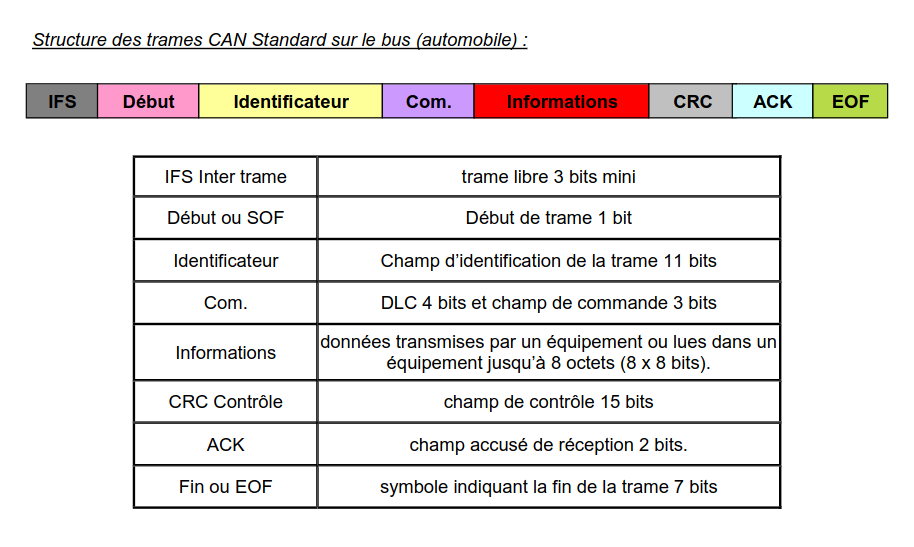
\includegraphics[width=.7\textwidth]{./images/structure_trames_CAN.png}
    \caption{Structure des trames CAN, source: \cite{exxotest}}
    \label{fig:structure_trames_CAN}
\end{figure}

\subsubsection*{Donner le nombre d'ID différents présents sur chaque bus identifiés (exports de donnéés depuis le logiciel MuxTrace).}

Pour les 3 bus étudiés (I/S, CONF, et CAR), le nombre d'ID différents présents sur chaque bus est respectivement de 22, 70 et 23.

% --------------------------------------------------------------------------------------------------------
% 1.2 Port OBDII
% --------------------------------------------------------------------------------------------------------

\subsection{Port OBDII}

\subsubsection*{A quoi sert le port OBDII ?}

Comme décrit sur le site \cite{klavkarr}, la norme OBDII a été instaurée à l'origine par la CARB, ``Californian Air Resources Board'' pour son acronyme en anglais, afin de surveiller les émissions polluantes des véhicules. La norme requiert que le véhicule surveille de manière continue le bon fonctionnement du moteur tout au long de sa durée de vie.\pagebreak

Le protocole OBD permet le diagnostic embarqué d'un véhicule. C'est un système électronique responsable de l'auto-diagnostic et de la production de rapports destinés aux professionnels de la réparation. Grâce à ce système, les techniciens ont accès à des informations sur les sous-systèmes du véhicule, permettant ainsi le suivi de sa performance et l'analyse des besoins en réparations.

Certaines versions de la norme OBDII sont énumérées ci-dessous.
\begin{itemize}
    \item L'OBD ou OBDI standardise le connecteur pour assurer son uniformité sur tous les véhicules. En revanche, le protocole de communication demeure plus ou moins spécifique en fonction des marques.
    \item L'OBDII est arrivé aux États-Unis en 1996 pour spécifier des protocoles communs. En plus de cela, contrairement à l'OBDI qui est connecté à l'extérieur de la console d'une voiture, l'OBDII est intégré au véhicule.
    \item L'EOBD, pour European OBD, reprenant l'OBDII, est spécifique pour les véhicules européens.
\end{itemize}
    
\subsubsection*{Reccherche bibliographique sur le web : câblage de connecteur, mode d'échange entre les outils et le véhicle.}

Comme on peut le voir à l'annexe \ref{fig:Port_OBDII}, le port OBDII est composé de 16 broches, chacune ayant un rôle spécifique. Parmi elles, il y a :

\begin{itemize}
    \item 2 broches pour le positif et le négatif du J1850 (SAE) utilisant le protocole de modulation de durée d'impulsion (VPW).
    \item 2 broches pour récupérer la masse du châssis et la masse du signal.
    \item 2 broches pour la ligne K et la ligne L utilisant un protocole de communication série asynchrone.
    \item 2 broches pour le LOW et le HIGH du protocole CAN.
    \item 7 broches non standard réservées au constructeur.
    \item 1 broche d'alimentation connectée à la batterie du véhicule pour alimenter les outils de scan. Elle est soit de type A avec une tension de 12V pour les voitures, ou de type B avec une tension de 24V pour les poids lourds.
\end{itemize}

Les informations sont générées par les unités de contrôle du moteur puis sont analysées par les outils connectés au port OBDII présent dans le véhicule.

% ========================================================================================================
% 2 Utilisation du logiciel MuxTrace
% ========================================================================================================

\section{TP1: Utilisation du logiciel MuxTrace}

Dans cette partie, nous allons utiliser le logiciel MuxTrace afin d'analyser les trames circulant dans les bus CAN. Pour cela, nous allons nous interfacer avec les bus I/S, CONF, et CAR grâce à la plaque de branchement de la maquette (voir illustration du branchement, annexe \ref{fig:tableau_interface}). Les signaux des bus CAN sont ensuite envoyés sur un boîtier USB-MUX-6C6L, avec le CAN CONF sur le port 1, le CAN I/S sur le port 2, et le CAN CAR sur le port 3 (voir illustration annexe \ref{fig:boitier_usb}). Cela permet, au final, de récupérer les informations des trames sur le logiciel MuxTrace. \pagebreak

Sur le logiciel MuxTrace, nous configurons chaque bus avec le bon débit en utilisant la détection automatique, comme illustré dans la figure \ref{fig:detection_auto_debit}.

\begin{figure}[H]
    \centering
    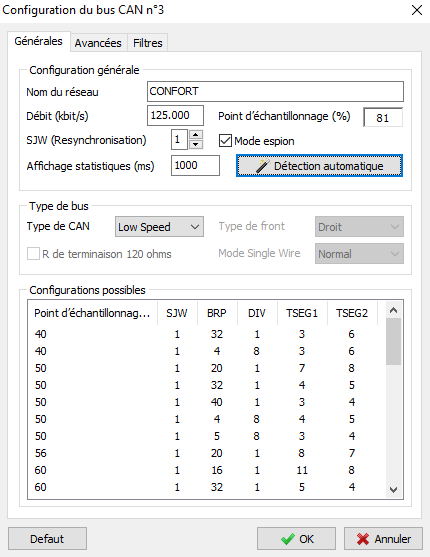
\includegraphics[width=.5\textwidth]{./images/detection_auto_debit.PNG}
    \caption{Outil de détection automatique du débit sur le logiciel MuxTrace.}
    \label{fig:detection_auto_debit}
\end{figure}

Nous pouvons ensuite observer les trames pour les 3 bus CAN sur le logiciel MuxTrace, comme on peut le voir dans la figure \ref{fig:liste_trames_bus}.

\begin{figure}[H]
    \centering
    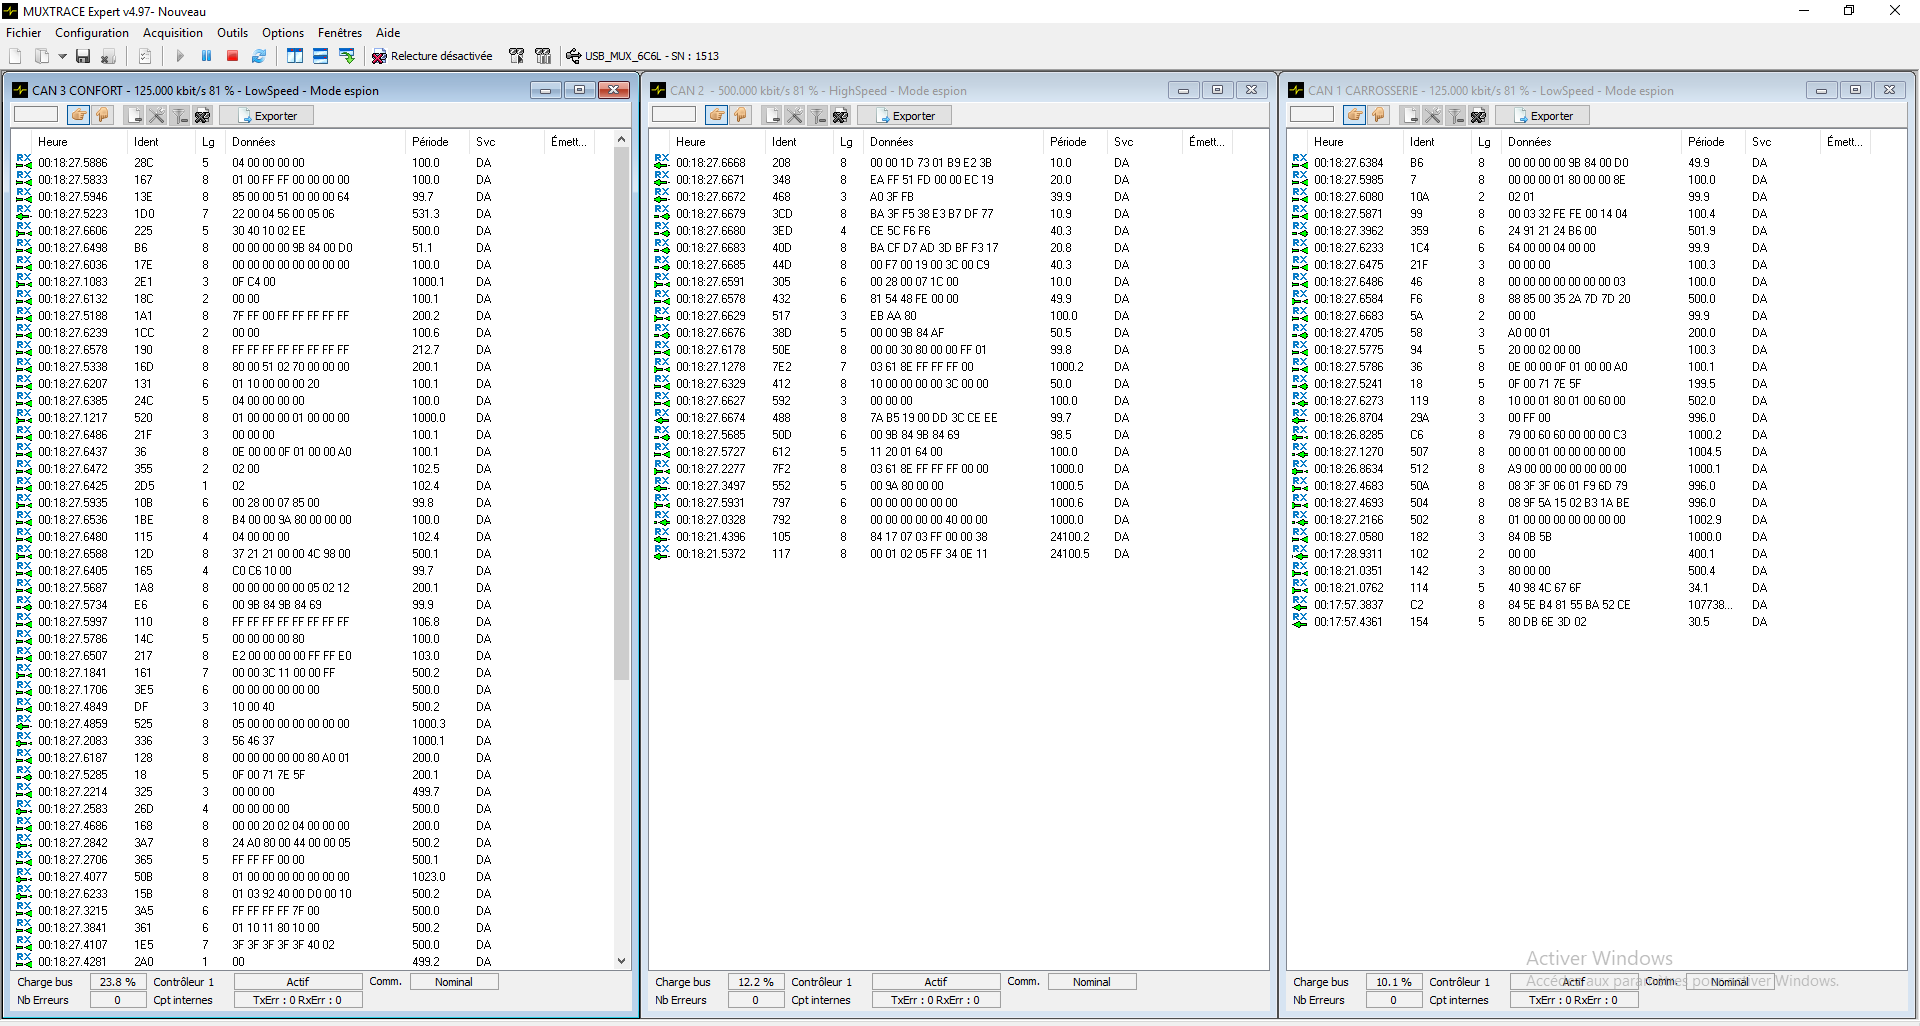
\includegraphics[width=\textwidth]{./images/liste_trames_bus.PNG}
    \caption{Observation des trames sur le logiciel MuxTrace.}
    \label{fig:liste_trames_bus}
\end{figure}

% --------------------------------------------------------------------------------------------------------
% 2.3 Etude practique : régime moteur
% --------------------------------------------------------------------------------------------------------

\subsection{Etude pratique : régime moteur}

\subsubsection*{Observer sur le bus IS la trame 208.}

Sur MuxTrace nous pouvons voir que la trame d'ID 208 du bus IS contient des données de 8 octets et emets avec une période de 10ms.

\subsubsection*{Faites varier le régime moteur et donnez vos observations sur le champs de données. Par exemple, vous pouvez faire varier la vitesse par pas de 1000tr.min\textsuperscript{-1}.}

Lorsque nous faisons varier le régime moteur, nous constatons que le premier octet de la trame 208 varie. Nous avons reporté dans le tableau \ref{tab:regime_moteur_trame_208} la valeur du premier octet obtenue en faisant varier la vitesse par pas de 1000tr.min\textsuperscript{-1} de 0tr.min\textsuperscript{-1} à 5000tr.min\textsuperscript{-1}.

\begingroup
\begin{table}[H]
    \centering
    \begin{tabular}{c c c}
        \toprule
        \makecell{\textbf{Régime moteur}\\ \textbf{(tr.min\textsuperscript{-1})}} & \makecell{\textbf{Premier octet}\\ \textbf{(hexa)}} & \makecell{\textbf{Premier octet}\\ \textbf{(base 10)}} \\
        \midrule
        0    & 00 & 00 \\
        1000 & 21 & 33 \\
        2000 & 3F & 63 \\
        3000 & 5E & 94 \\
        4000 & 7D & 125 \\
        5000 & 9B & 155 \\
        \bottomrule
    \end{tabular}
    \caption{Premier octet de la trame 208 en fonction du régime moteur.}
    \label{tab:regime_moteur_trame_208}
\end{table}
\endgroup

\subsubsection*{Pouves-vous en déduire une suite logique sur la variation du régime moteur ? Dans tous les cas, donnez vos arguments.}

En observant les valeurs en base 10, on constate la suite suivante:

\begin{itemize}
    \item de 0 à 1000: +33
    \item de 1000 à 2000: +30
    \item de 2000 à 3000: +31
    \item de 3000 à 4000: +31
    \item de 4000 à 5000: +30
\end{itemize}

On a donc une suite logique d'environ 31 par pas de 1000tr.min\textsuperscript{-1}.

% --------------------------------------------------------------------------------------------------------
% 2.2 Etude practique : vitesse véhicule
% --------------------------------------------------------------------------------------------------------

\subsection{Etude pratique : vitesse véhicule}

\subsubsection*{Sur le bus IS, identifiez la ou les trames qui évolent en fonction de la vitesse du véhiule.}

Lorsque l'on modifie la vitesse, nous constatons un changement sur le premier, troisième et cinquième octet de la trame 44D ainsi que le premier octet de la trame 38D.

\subsubsection*{Observez la trame 0x44D. Quelle est sa taille et sa fréquence ?}

La trame 0x44D a une taille de 8 octets et une fréquence de 40ms

\subsubsection*{Faites varier la vitesse du véhicle et donnez vos observations sur les champs de données. Par exemple, vous pouvez fair varier la viteese par pas de 10 de 0 à 100Km/h.}

Lorsque nous faisons varier la vitesse du véhicule, nous constatons que le premier, troisième et cinquième octet de la trame 44D varient avec la même valeur. Nous avons reporté dans le tableau \ref{tab:vitesse_vehicule_trame_44D} la valeur obtenue en faisant varier la vitesse par pas de 10km/h de 0km/h à 100km/h.

\begingroup
\begin{table}[H]
    \centering
    \begin{tabular}{c c c}
    \toprule
    \makecell{\textbf{Vitesse véhicule}\\ \textbf{(km/h)}} & \makecell{\textbf{Octets 1,3 et 5}\\ \textbf{(hexa)}} & \makecell{\textbf{Octets 1,3 et 5}\\ \textbf{(base 10)}} \\
    \midrule
    0  & 00 & 00 \\
    10 & 03 & 03 \\
    20 & 08 & 08 \\
    30 & 0B & 11 \\
    40 & 0F & 15 \\
    50 & 13 & 19 \\
    60 & 17 & 23 \\
    70 & 1B & 27 \\
    80 & 1E & 30 \\
    90 & 22 & 34 \\
    100& 26 & 38 \\
    \bottomrule
    \end{tabular}
    \caption{Octets 1, 3 et 5 de la trame 44D en fonction de la vitesse du véhicule.}
    \label{tab:vitesse_vehicule_trame_44D}
\end{table}
\endgroup

\subsubsection*{Pouvez-vous en déduire une suite logique sur la variation de la vitesse du véhicule ? Dans tous les cas, donnez vos arguments.}

En observant les valeurs en base 10, on constate une suite logique de 3.8, soit environ 4 par pas de 10km/h.

% --------------------------------------------------------------------------------------------------------
% 2.3 Etude practique : Comodo de phares
% --------------------------------------------------------------------------------------------------------
\subsection{Etude pratique : Comodo de phares}

\subsubsection*{Quels identificateurs de trames ont un rapport avec les commandes d'éclairage, de signalisation et d'essuyage ?}

Lorsque nous actionnons les commandes d'éclairage, de signalisation ou d'essuyage, nous observons des changements sur la trame 94, avec le premier octet commandant l'éclairage, le deuxième les essuie-glaces et le troisième la signalisation.

\subsubsection*{Sur quels bus avez-vous observé ces identificateurs ?}

Nous observons que la trame 94 circule sur le bus carrosserie.

\subsubsection*{Quelle est la taille de la trame concernée ?}

La taille de la trame 94 est de 5 octets.

\subsubsection*{Actionnez la commande d'éclairage et établissez un tableau des fonctions comandées.}

Après avoir fait varier la commande d'éclairage entre feux de position, feux de croisement, feux de route et anti-brouillard, nous avons reporté dans le tableau \ref{tab:commande_eclairage_trame_94} les valeurs prises par le premier octet de la trame 94.

\begingroup
\begin{table}[H]
    \centering
    \begin{tabular}{c c}
    \toprule
    \makecell{\textbf{fonction comandée}} & \makecell{\textbf{Premier octet}\\ \textbf{(hexa)}} \\
    \midrule
    Feux éteints  & 20 \\
    Feux de position  & 40 \\
    Feux de croisement & 80 \\
    Feux de route & 98 (au moment de l'activation) \\
    Anti-brouillard & 84 (au moment de l'activation) \\
    Appel de phare & 28 (au moment de l'activation) \\
    \bottomrule
    \end{tabular}
    \caption{Premier octet de la trame 94 en fonction de la commande d'éclairage.}
    \label{tab:commande_eclairage_trame_94}
\end{table}
\endgroup

% --------------------------------------------------------------------------------------------------------
% 2.4 Etude practique : Rétroviseurs
% --------------------------------------------------------------------------------------------------------

\subsection{Etude pratique : Rétroviseurs}

\subsubsection*{Faites fonctionner les rétroviseurs du côté droit et du côté gauche, et soyez attentif aux trames. Quel est l'identificateur de trame correspond aux rétroviseurs gauche et droit ?  Sur quel bus avez-vous fait l'observation ?}

Lorsque nous faisons fonctionner les rétroviseurs avec le sélecteur et les boutons directionnels, nous constatons des changements sur la trame 115. Cette trame est présente sur le bus confort.

\subsubsection*{Quelle est la taille des données de cette trame ?}

La trame 115 a une taille de 4 octets.

\subsubsection*{A quoi sert le premier octet de donnée ?}

En observant la trame 115, nous constatons que les 4 premiers bits du premier octet contrôlent la direction et les 4 derniers bits du deuxième octet contrôlent le choix entre le rétroviseur gauche et droit.

\subsubsection*{Observer le premier octet de donnnés et établissez un tableau des actions  réalisées en fonction de la valeur de l'octet.}

Nous avons reporté les actions réalisées en fonction des 4 premiers bits du premier octet dans le tableau \ref{tab:direction_trame_115} et ceux des 4 derniers bits du premier octet dans le tableau \ref{tab:choix_retro_trame_115}.

\begingroup
\begin{table}[H]
    \centering
    \begin{tabular}{c c}
    \toprule
    \makecell{\textbf{Actions réalisées}} & \makecell{\textbf{4 premier bits}\\ \textbf{(hexa)}} \\
    \midrule
    Aucune direction  & 0 \\
    Bas & 1 \\    
    Haut  & 2 \\
    Gauche & 4 \\
    Droite & 8 \\
    \bottomrule
    \end{tabular}
    \caption{Direction du rétroviseur en fonction de la valeur des 4 premiers bits du premier octet.}
    \label{tab:direction_trame_115}
\end{table}
\endgroup

\begingroup
\begin{table}[H]
    \centering
    \begin{tabular}{c c}
    \toprule
    \makecell{\textbf{Actions réalisées}} & \makecell{\textbf{4 derniers bits}\\ \textbf{(hexa)}} \\
    \midrule
    Aucun selectionné  & 1 \\
    rétroviseur droit & 2 \\    
    rétroviseur gauche  & 4 \\
    \bottomrule
    \end{tabular}
    \caption{Choix du rétroviseur en fonction de la valeur des 4 derniers bits}
    \label{tab:choix_retro_trame_115}
\end{table}
\endgroup

\subsubsection*{Utiliser le générateur interactif afin d'émettre la trame de commande des rétroviseurs observée précédemment. Vérifiez les trames de commandes observées précédemment en associant des touches de votre clavier pour piloter les rétroviseurs. Vous pouvez faire de même avec les lève-vitres ?}

Pour pouvoir utiliser le générateur interactif sur le logiciel MuxTrace, nous devons tout d'abord l'activer pour le bus CAN, comme montré dans la figure \ref{fig:generateur_interactif_activation}.


\insererfigure{./images/activer_generateur.PNG}{.7}{Activation du générateur intéractif pour le bus CAN sur MuxTrace}{generateur_interactif_activation}

Nous pouvons ensuite ouvrir le générateur interactif de trames CAN via le menu déroulant "Fenêtres", comme illustré dans la figure \ref{fig:ouvrir_generateur}.

\insererfigure{./images/ouvrir_generateur.png}{.7}{Ouvrir le générateur intéractif de trames CAN sur MuxTrace}{ouvrir_generateur}

Nous avons ensuite créé une trame d'ID 115 avec comme données 82 00 00 00, ce qui correspond à actionner le rétroviseur droit vers la droite. Cette trame est émise sur le bus confort, qui correspond au CAN 3 dans notre cas. De plus, nous avons configuré la touche "U" du clavier pour émettre la trame. La trame créée est illustrée à la figure \ref{fig:generateur_retro_droit}.

\insererfigure{./images/generateur_retro_droit.PNG}{.7}{Trame de contrôle du rétroviseur droit crée dans le générateur intéractif}{generateur_retro_droit}

% --------------------------------------------------------------------------------------------------------
% 2.5 Etude practique : Faites votre choix
% --------------------------------------------------------------------------------------------------------

\subsection{Etude pratique : Faites votre choix}

\subsubsection*{En fonction de votre avancement dans la séance de TP, vous pouvez exposer une ou deux trames supplémentaires de votre choix sur une ou plusieurs bus de la maquette. De la même manière que précédemment, donnez la taille de données, vos observations sous forme de tableau et justifiez vos analyses.}

- Commande radio:

Nous allons dans cette partie déterminer la trame responsable des commandes radio. Pour cela, nous avons actionné les commandes radio à partir des boutons sous le volant et nous avons observé un changement sur la trame 21F du bus CAN carrosserie, notamment sur le premier octet. Nous avons reporté les commandes radio en fonction du premier octet de la trame 21F dans le tableau \ref{tab:commande_radio_trame_21F}.

\begingroup
\begin{table}[H]
    \centering
    \begin{tabular}{c c}
    \toprule
    \makecell{\textbf{Actions réalisées}} & \makecell{\textbf{Premier octet}\\ \textbf{(hexa)}} \\
    \midrule
    SRC & 02 \\
    Augmentation volume & 08 \\    
    Diminution volume & 04 \\
    Station suivante & 80 \\
    Station précedente & 40 \\
    \bottomrule
    \end{tabular}
    \caption{Commande radio en fonction de la valeur du premier octet de la trame 21F}
    \label{tab:commande_radio_trame_21F}
\end{table}
\endgroup




% ========================================================================================================
% 3 Utilisation du logiciel MuxTrace et DBEdit
% ========================================================================================================

\section{TP2: Utilisation du logiciel MuxTrace et DBEdit}

\subsubsection*{Basé sur les observations faites dans la section précédente, créer une base de donnée pour chaque bus et chaque identifiant de paquets analysées.}

À partir de ce qui était obtenu précédemment, une base de données est créé, qui comportera toutes les trames importantes étudiées.
Voici ci-dessous un exemple \ref{fig:regime_db} de création de trame, dans cet exemple ce sera la trame liée au régime :

\begin{figure}[H]
    \centering
    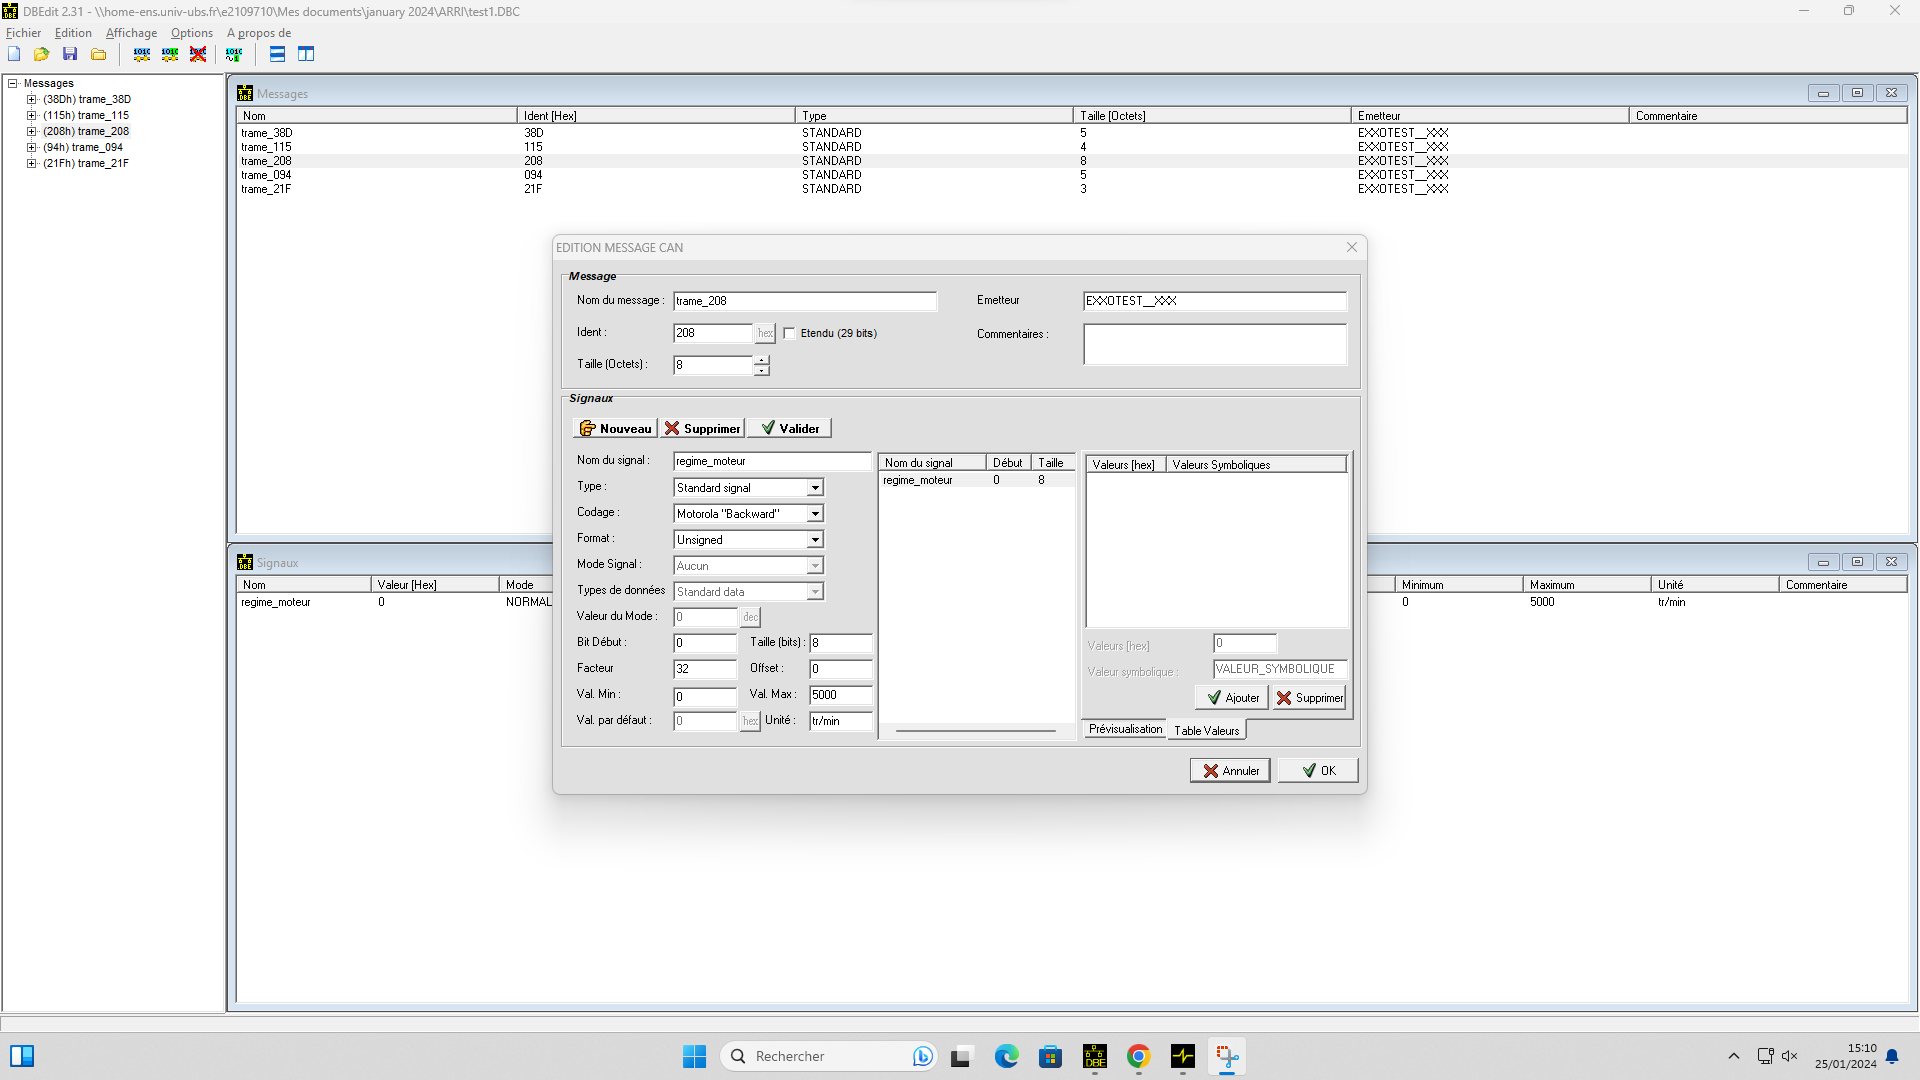
\includegraphics[width=.7\textwidth]{./images/Regime_DB.png}
    \caption{Création de trame DBEdit.}
    \label{fig:regime_db}
\end{figure}

Il y a plusieurs choses que nous pouvons observer sur cette liste :

\begin{itemize}
    \item Tout d'abord on doit donner l'identité de la trame qui correspond dans ce cas-ci à celle du régime moteur (208).
    \item Ensuite on donne le nombre d'octets que contient la trame (8, dans cet exemple).
    \item Après cela on ajoute  une valeur maximale et minimale (de 0 à 5000, dans cet exemple).
    \item On peut aussi ajouter un offset si on en a besoin (0, dans cet exemple)
    \item La dernière chose qui a changé est le "Facteur", qui représente le pas moyen entre chaque valeur (1000 tr/min dans ce cas).
\end{itemize}

\subsubsection*{Lorsque les fichiers de base de données sont prêts, chagez-les depuis votre projet MuxTrace. Vérifiez que vos observations sont cohérentes lorsque vous actionnez les différentes commandes concernées de la maquette.}

Une fois toutes les trames ajoutées dans la base de données sur DB Edit, on va utiliser MuxTrace dans le but d'observer que nos choix lors de la création de cette dernière sont cohérents.
Après avoir ajouté notre base de données on viendra changer quelques actionneurs sur la maquette, qui sont bien sûrs en lien avec les trames ajouté dans notre base de données, comme par exemple la trame liée au régime moteur.

Grâce à ça, on a pu vérifier que notre base de données correspondait avec ce qui est fait via la maquette.

\subsubsection*{Qu'en déduisez-vous de l'intéret de ces bases de données ?}

L'intérêt des bases de données, est de repérer les trames que nous voulons étudier pour ensuite agir dessus et vérifier que nous obtenons bien le comportement souhaité.

\subsubsection*{Utilisez maintenant le générateur interactif de MuxTrace pour faire varier les champs de données d'un ID de trame connu dans la base de données. Quel est l'intéret de ce lien avec la base de donnée par rapport aux signaux d'une trame ?}

Pour cette question dans MuxTrace, on ajoute un générateur interactif, avec ce dernier, on viendra faire varier certaines trames pour ensuite vérifier si on bien le bon rendu sur la maquette.
Donc par exemple si on augmente la trame correspondant au régime moteur alors sur la maquette on pourra aussi observer une augmentation.
Une fois cela fait on vérifie si les valeurs que nous avons définies lors de la création de la base de données son juste ou non, en comparant tout simplement la valeur espérée  valeur réelle lue sur la maquette.
En fonction du résultat on ajuste ou non notre "facteur", par exemple.
Voici si un exemple \ref{fig:DB_MuxTrace} de DBEdit dans MuxTrace : 

\begin{figure}[H]
    \centering
    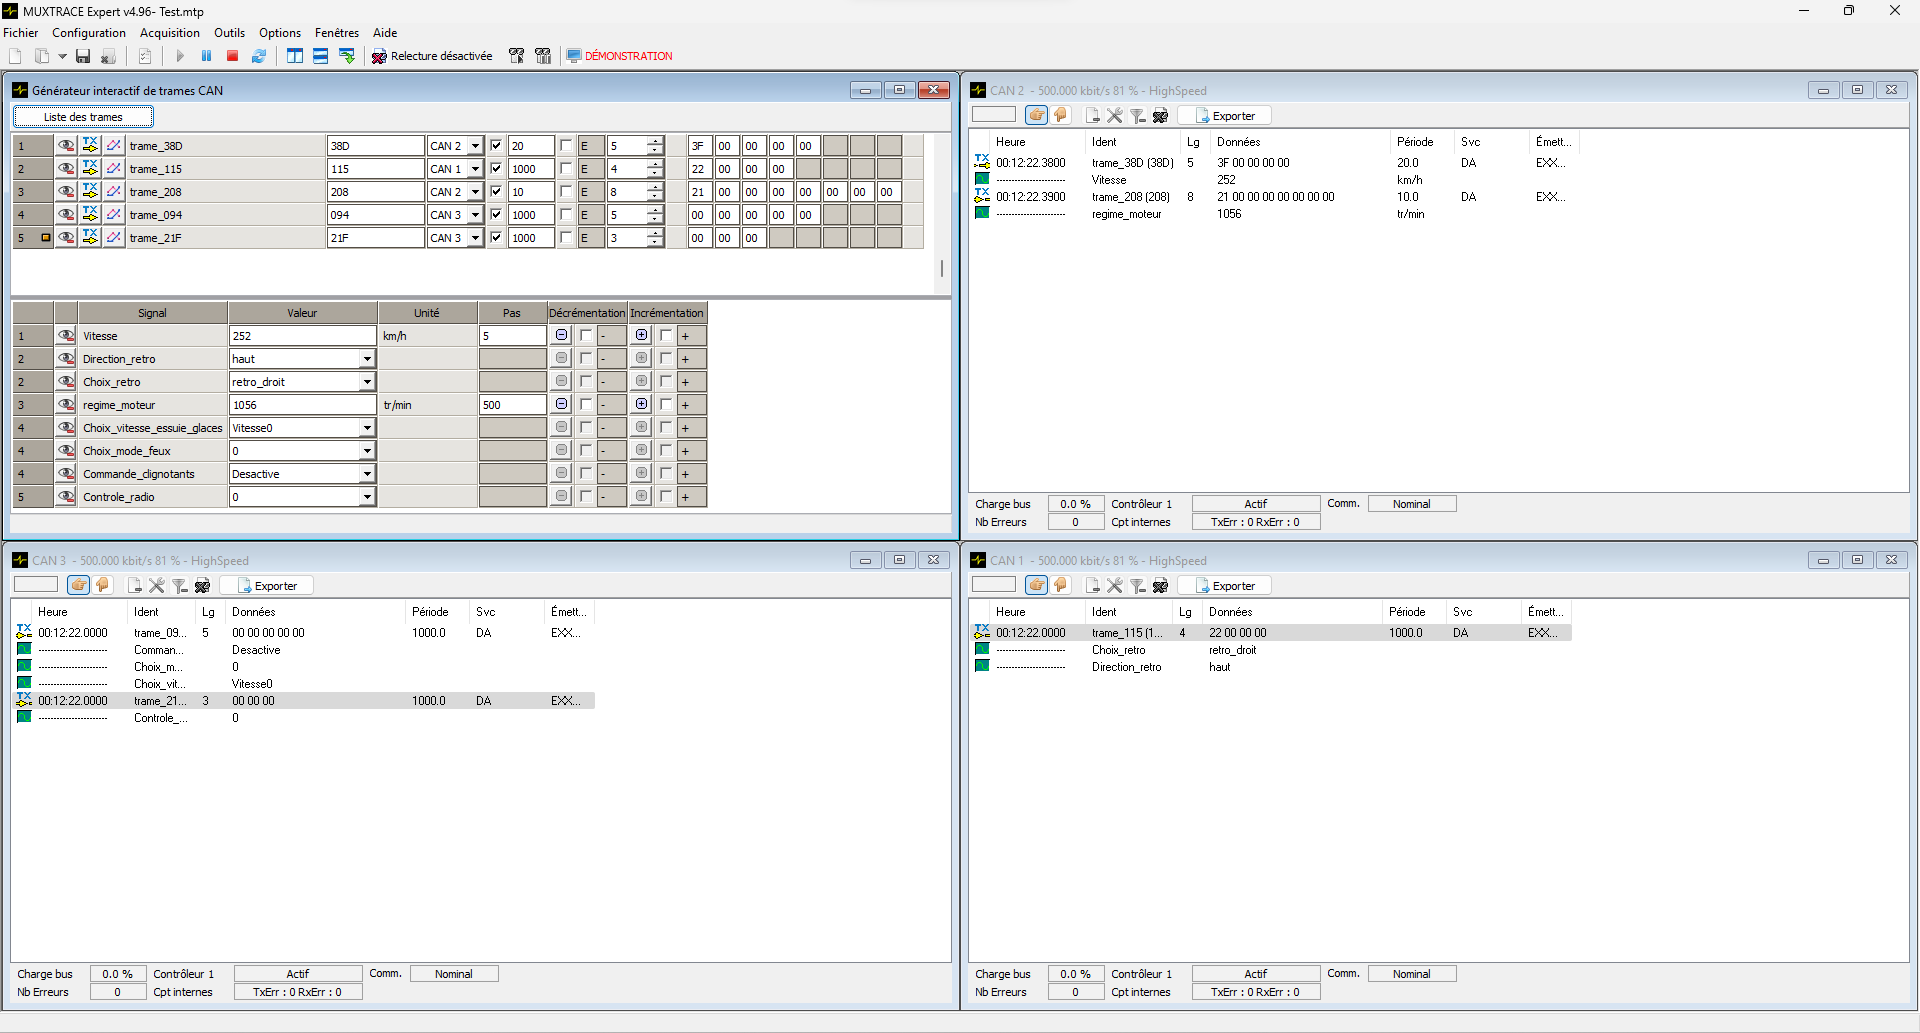
\includegraphics[width=.9\textwidth]{./images/MUXTRACE_with_DB.png}
    \caption{Utilisation d'une base de donnée DBEdit sur MuxTrace.}
    \label{fig:DB_MuxTrace}
\end{figure}


On peut observer dans le cas ci-dessus qu'on a notre base de données avec nos trames à l'intérieur ainsi qu'une touche qui est affectée pour choisir si oui ou non ont envoyé sur le bus CAN une commande.
Mais il y a aussi bien d'option, par exemple nous ne sommes pas obligés à utiliser une touche mais plutôt d'envoyer de façon périodique une commande.
Une fois nos paramètres choisis, il nous reste les tests.

% ========================================================================================================
% 4 Utilisation du mode programmation sous MuxTrace
% ========================================================================================================

\section{TP3: Utilisation du mode programmation sous MuxTrace}

\textit{Sous MuxTrace, il est possible d'avoir un mode programmation qui permet d'automatiser la génération interactive de trames sur des actions clavier ou sur des évènements conditionnels liés à la configuration du véhicule.}

% --------------------------------------------------------------------------------------------------------
% 4.1 chargement d'un exemple
% --------------------------------------------------------------------------------------------------------

\subsubsection*{Etude practique : chargement d'un exemple}

\textit{Dans un premier temps, on vous demande de charger le fichier d'exemple de dll fournit en séances de TP dans l'outil MuxTrace.}

\textit{Analysez et observez cet example et donnez vos remarques sur le comportement et les interactions de cet exemple sur la maquete.}

La figure \ref{fig:MuxTrace_dll_default} montre le bon fonctionnement du programme MuxTrace après sa configuration avec l'exemple de fichier .dll sans aucune configuration supplémentaire.

Dans l'Annexe \ref{sec:annexeB} - Code \ref{lst:onevent} se trouve le code original de la fonction OnEvenet chargée de mettre à jour périodiquement les données de chaque trame sur les trois bus comme le montre la figure \ref{fig:MuxTrace_dll_default}.

\begin{figure}[H]
    \centering
    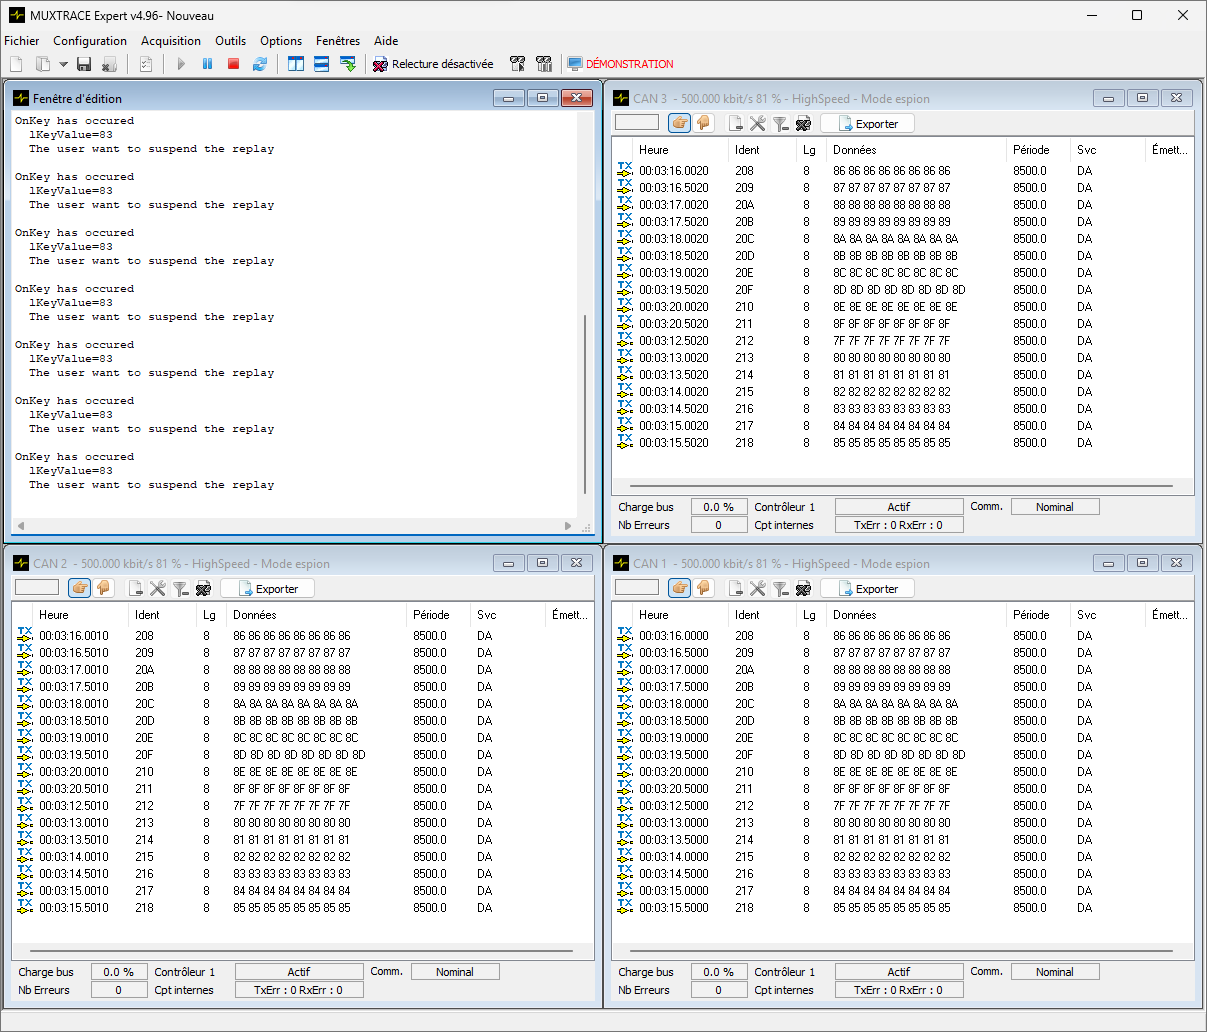
\includegraphics[width=0.95\textwidth]{./images/MuxTrace_dll_running_default_example_number_1_res_indus_31_01_2024_ubs_lorient_M1SESI.png}
    \caption{ss}
    \label{fig:MuxTrace_dll_default}
\end{figure}

% --------------------------------------------------------------------------------------------------------
% 4.2 Création de votre exemple
% --------------------------------------------------------------------------------------------------------

\subsubsection*{Etude practique : Création de votre exemple}

\textit{Proposez un scénario d'exemple que vous souhaitez réalisér et décrivez-le de manière détaillée (identifiants de paquets, évènements conditionnels, \dots). Ces précisions porteront une attention toute particulière pour évaluer le Compte-rendu de TP avec le code source et la dll qui sera remis en fin de séances de TPs.}

\textit{Développez votre programme en C en partant de l'exemple foruni dans le répertoire d'installation de MuxTrace afin de créers votre dll d'exmplequi réalisera le scénario que vous aurez inventé.}

En groupe, l'idée était de démontrer l'utilisation et la gestion correctes des châssis et des bus avec une relation entre action et réaction, c'est-à-dire qu'une action dans un système du simulateur de véhicule générera une réaction dans un autre système. De cette manière, la logique présentée dans la figure \ref{fig:OnCanEvent_UML} a été développée.

\begin{figure}[H]
    \centering
    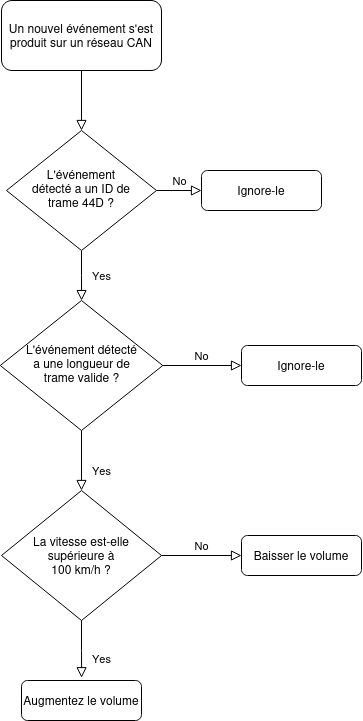
\includegraphics[width=.5\textwidth]{./images/OnCanEvent_UML.png}
    \caption{Diagramme UML du scénario proposé pour développer le test TP3.}
    \label{fig:OnCanEvent_UML}
\end{figure}

Pour réaliser la logique de la figure \ref{fig:OnCanEvent_UML} la fonction \textit{OnCanEvent} a été modifiée comme on peut le trouver dans l'Annexe \ref{sec:annexeB} - Code \ref{lst:oncanevent}.

En plus, dans l'annexe \ref{sec:annexeA}, dans la section \ref{sec:annexeA:TP3}, la figure \ref{fig:conf_additional_real_limit_vitesse} montre la configuration supplémentaire à effectuer dans MuxTrace pour l'implémentation du fichier `.dll'. En outre, les figures \ref{fig:test_local_1} et \ref{fig:test_local_2} montrent un avant et un après la modification manuelle de la valeur de la vitesse dans MuxTrace et le changement qu'elle produit dans l'image 44D (volume), ce qui permet de vérifier que le code développé fonctionne correctement.

\section{Conclusion}

Lors des différents TP que nous avons faits, nous avons utilisé une maquette qui représente une voiture avec tous ses accessoires qui lui sont liés. Cela nous permet donc de travailler avec un réseau de terrain, à savoir le bus CAN. Nous avons donc pu comprendre ce dernier avec tous les outils qui nous ont été fournis et qui ont été présentés précédemment.
Une fois la prise en main des différents outils effectuée, un script a été réalisé, que l'on peut voir dans le TP3.

\bibliographystyle{unsrt}
\bibliography{main.bib} 

% Ajout de l'annexe

\pagebreak

\appendix

\section{Annexe A : Illustration complémentaire}\label{sec:annexeA}

\subsection{TP1}

\begin{figure}[H]
    \centering
    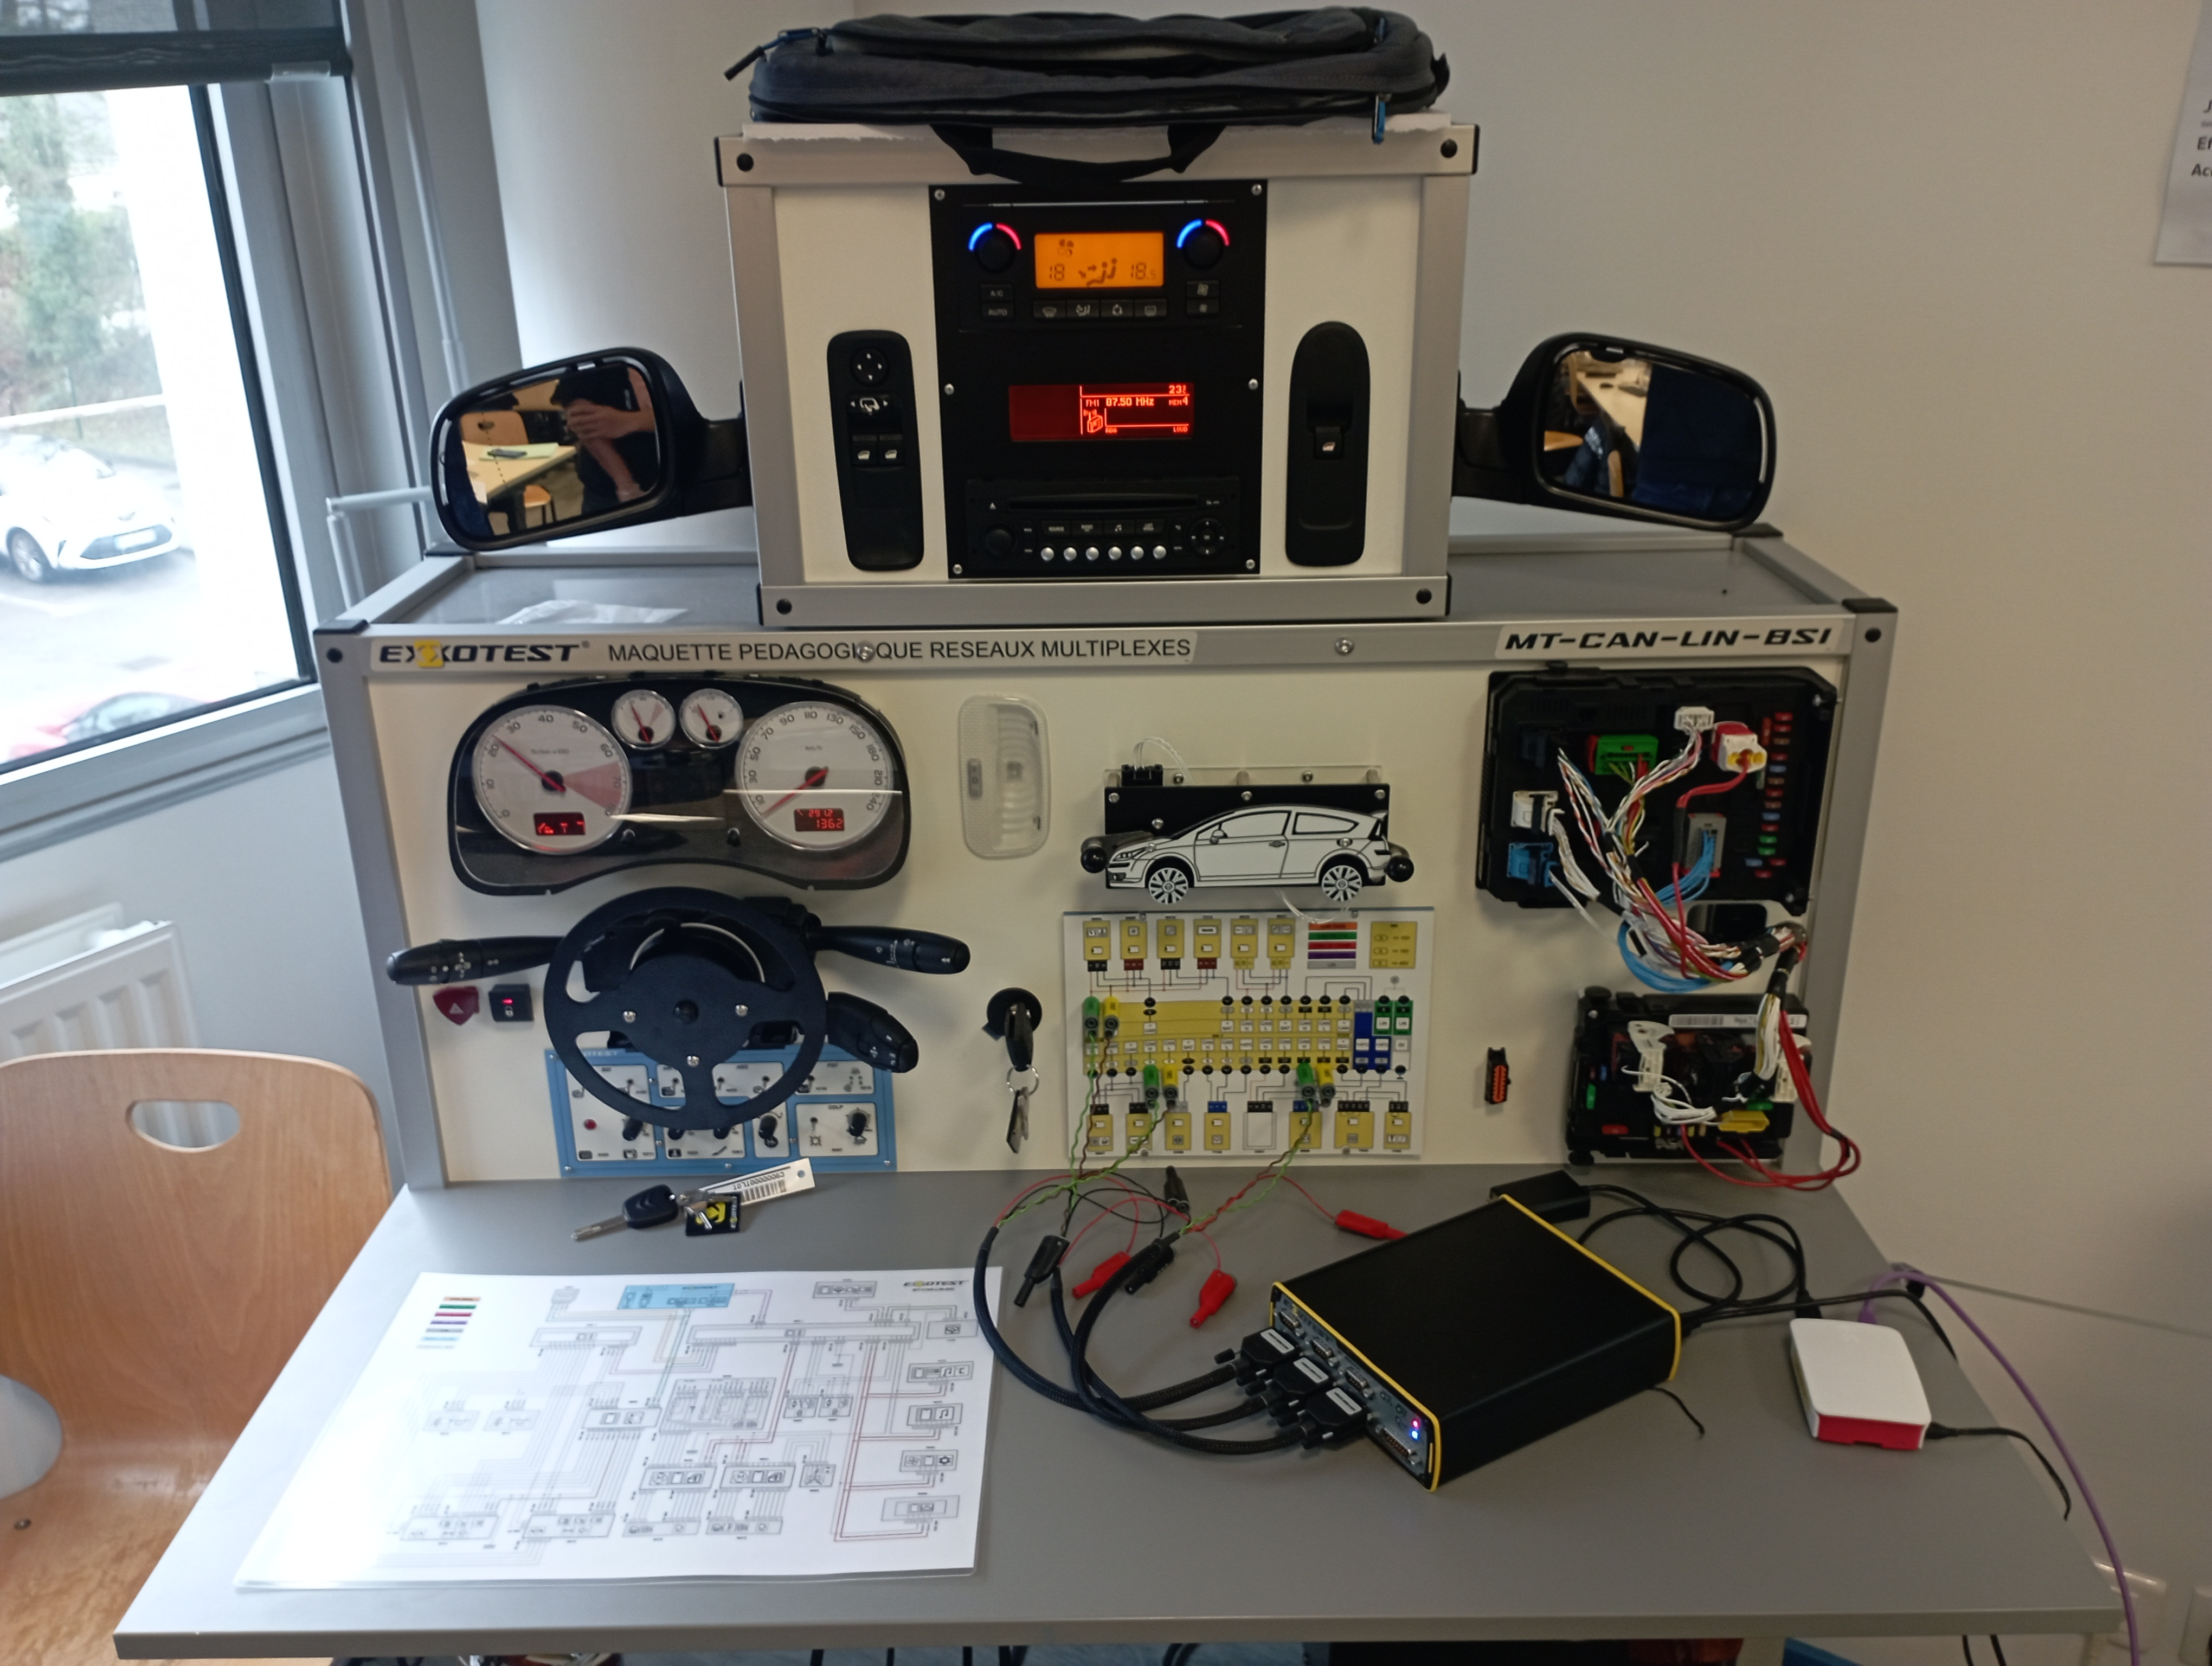
\includegraphics[width=.7\textwidth]{./images/maquette.jpg}
    \caption{Illustration de la maquette EXXOTEST.}
    \label{fig:maquette_EXXOTEST}
\end{figure}

\begin{figure}[H]
    \centering
    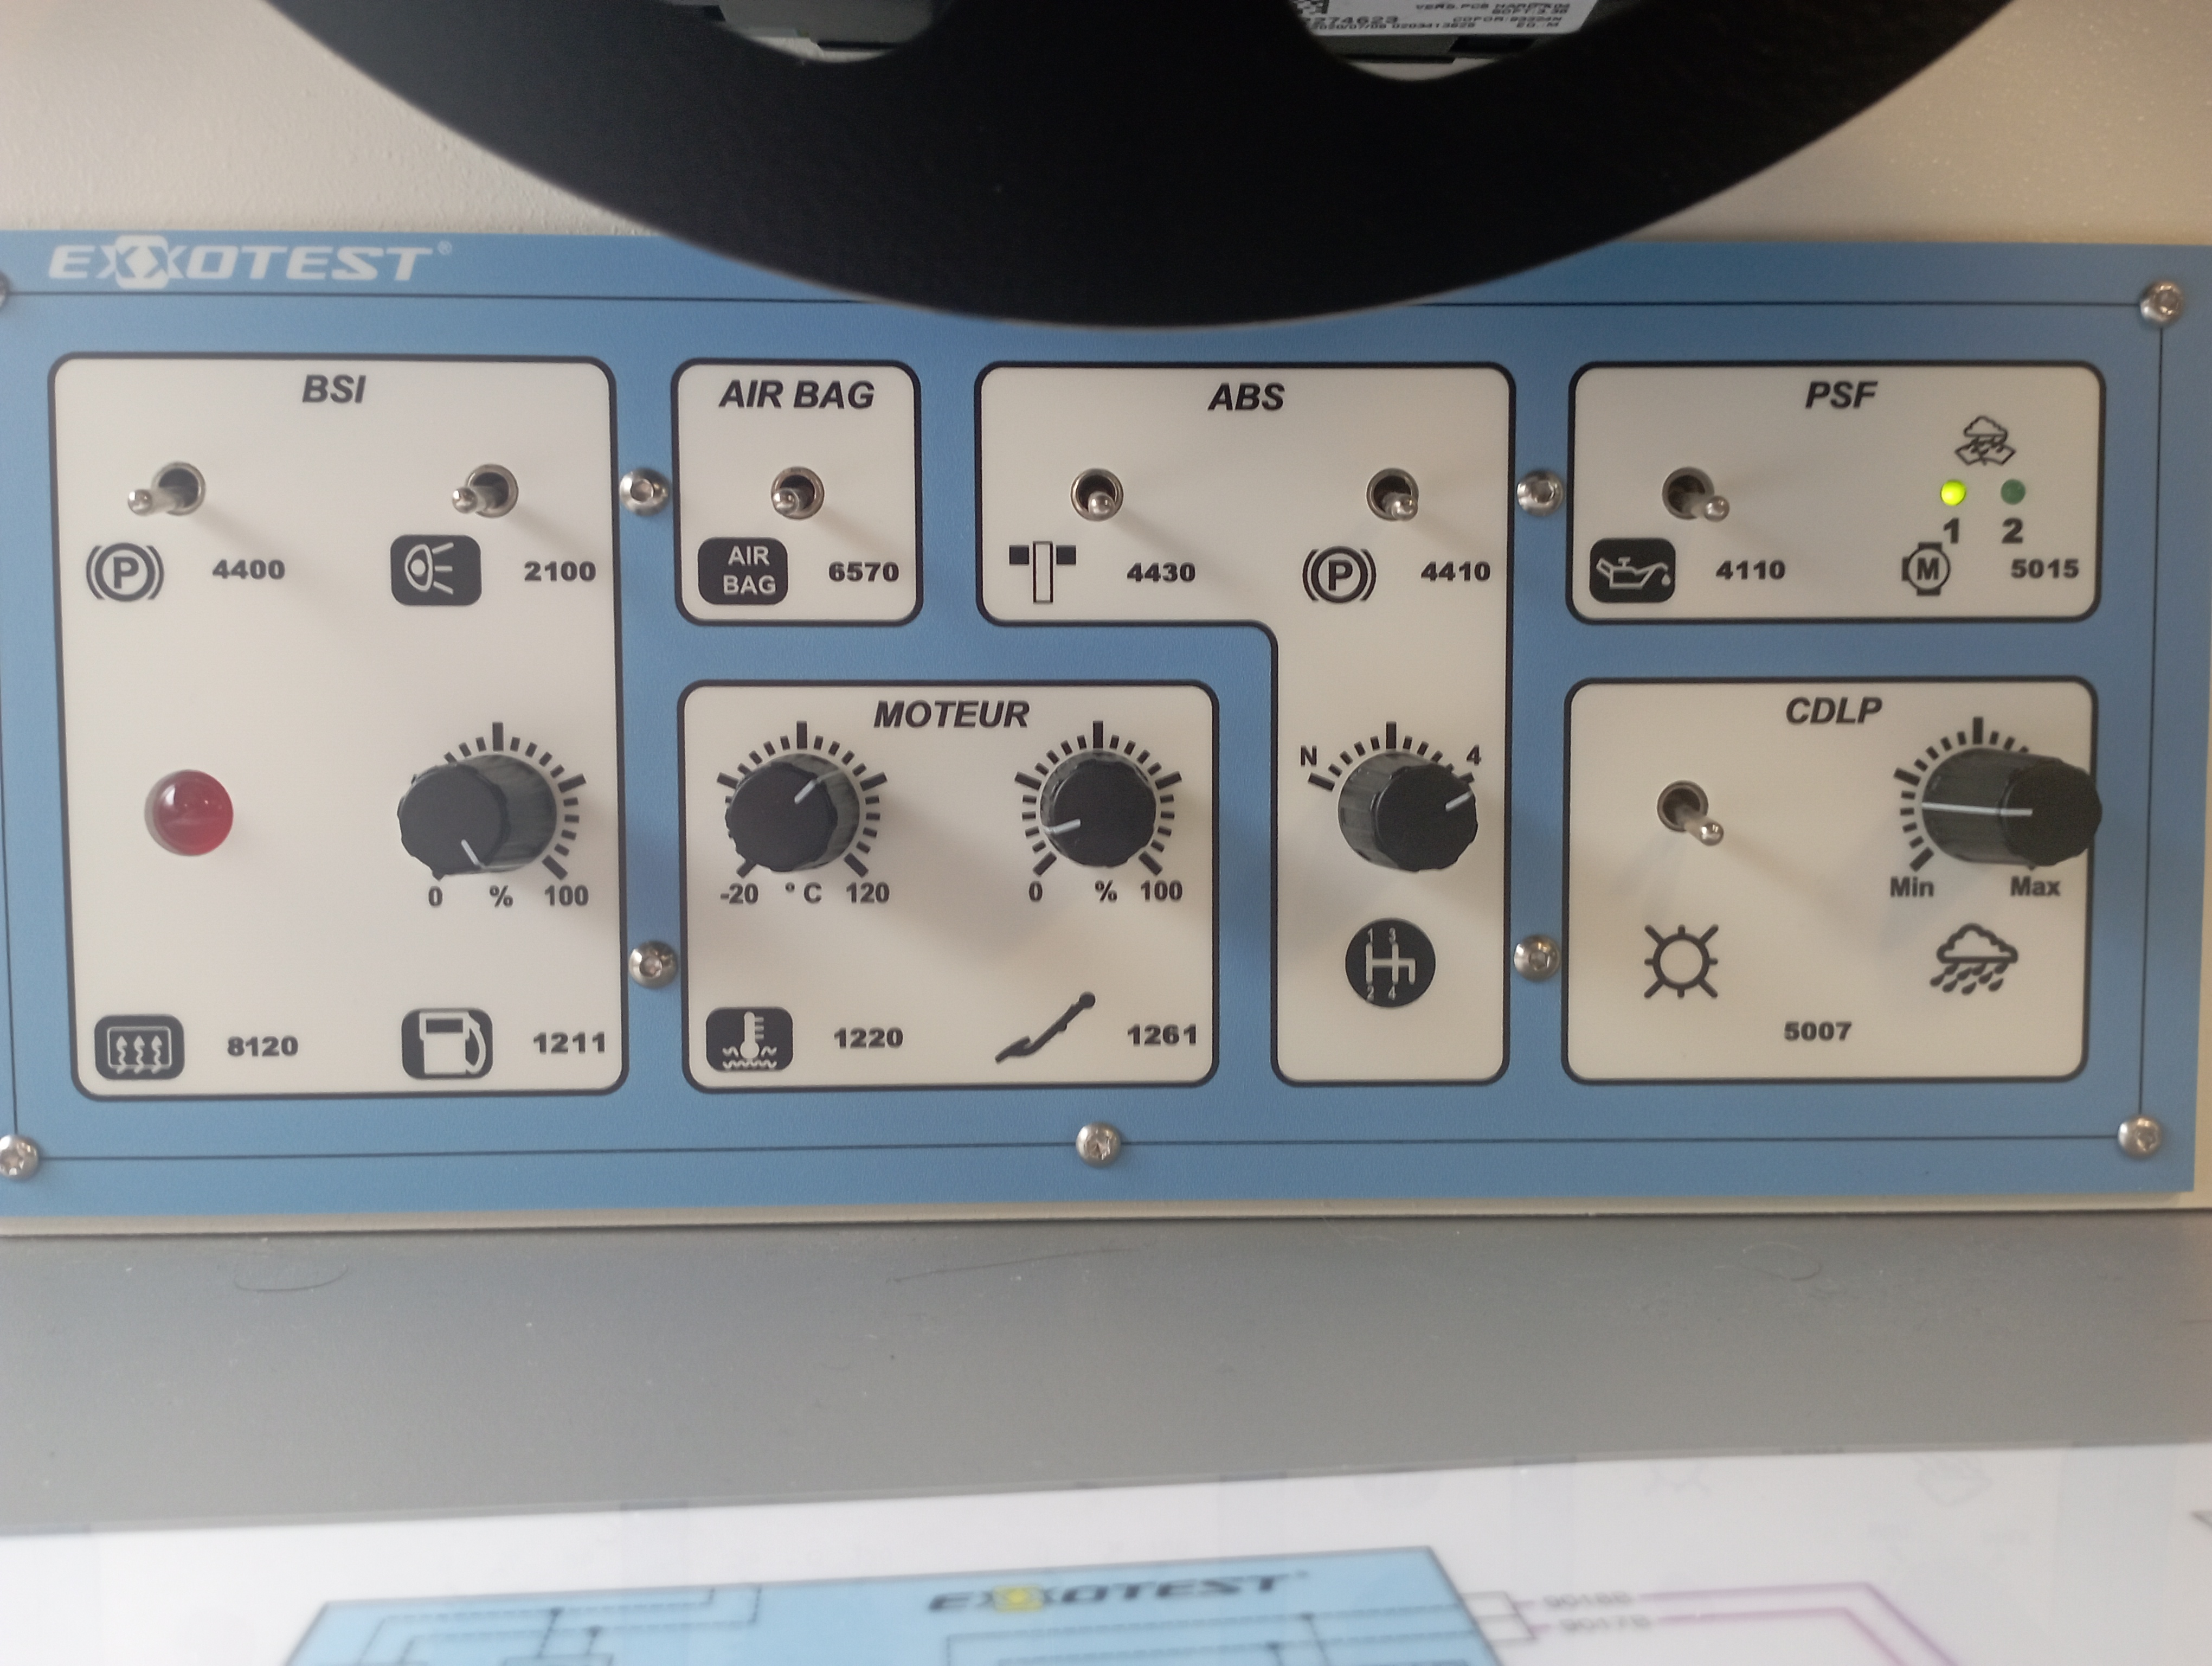
\includegraphics[width=.7\textwidth]{./images/potentiometres_simu.jpg}
    \caption{Illustration des potentiomètres et interrupteurs de la partie simulée.}
    \label{fig:potentiometres}
\end{figure}

\begin{figure}[H]
    \centering
    \includegraphics[width=.7\textwidth]{./images/schema_cablage.jpg}
    \caption{Schéma du cablage de la maquette.}
    \label{fig:schema_cablage}
\end{figure}

\begin{figure}[H]
    \centering
    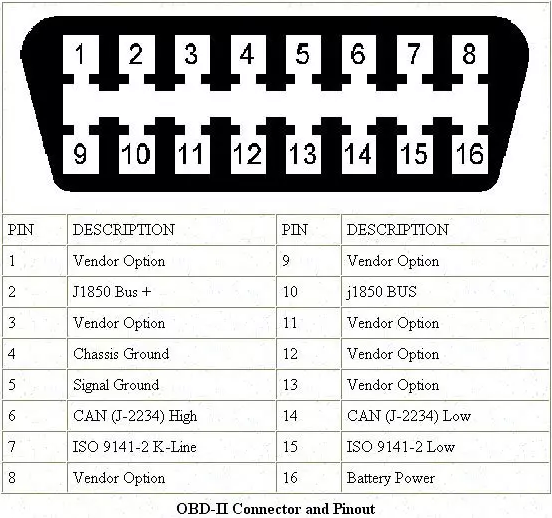
\includegraphics[width=.7\textwidth]{./images/OBDII_pins.png}
    \caption{Port OBDII.}
    \label{fig:Port_OBDII}
\end{figure}

\begin{figure}[H]
    \centering
    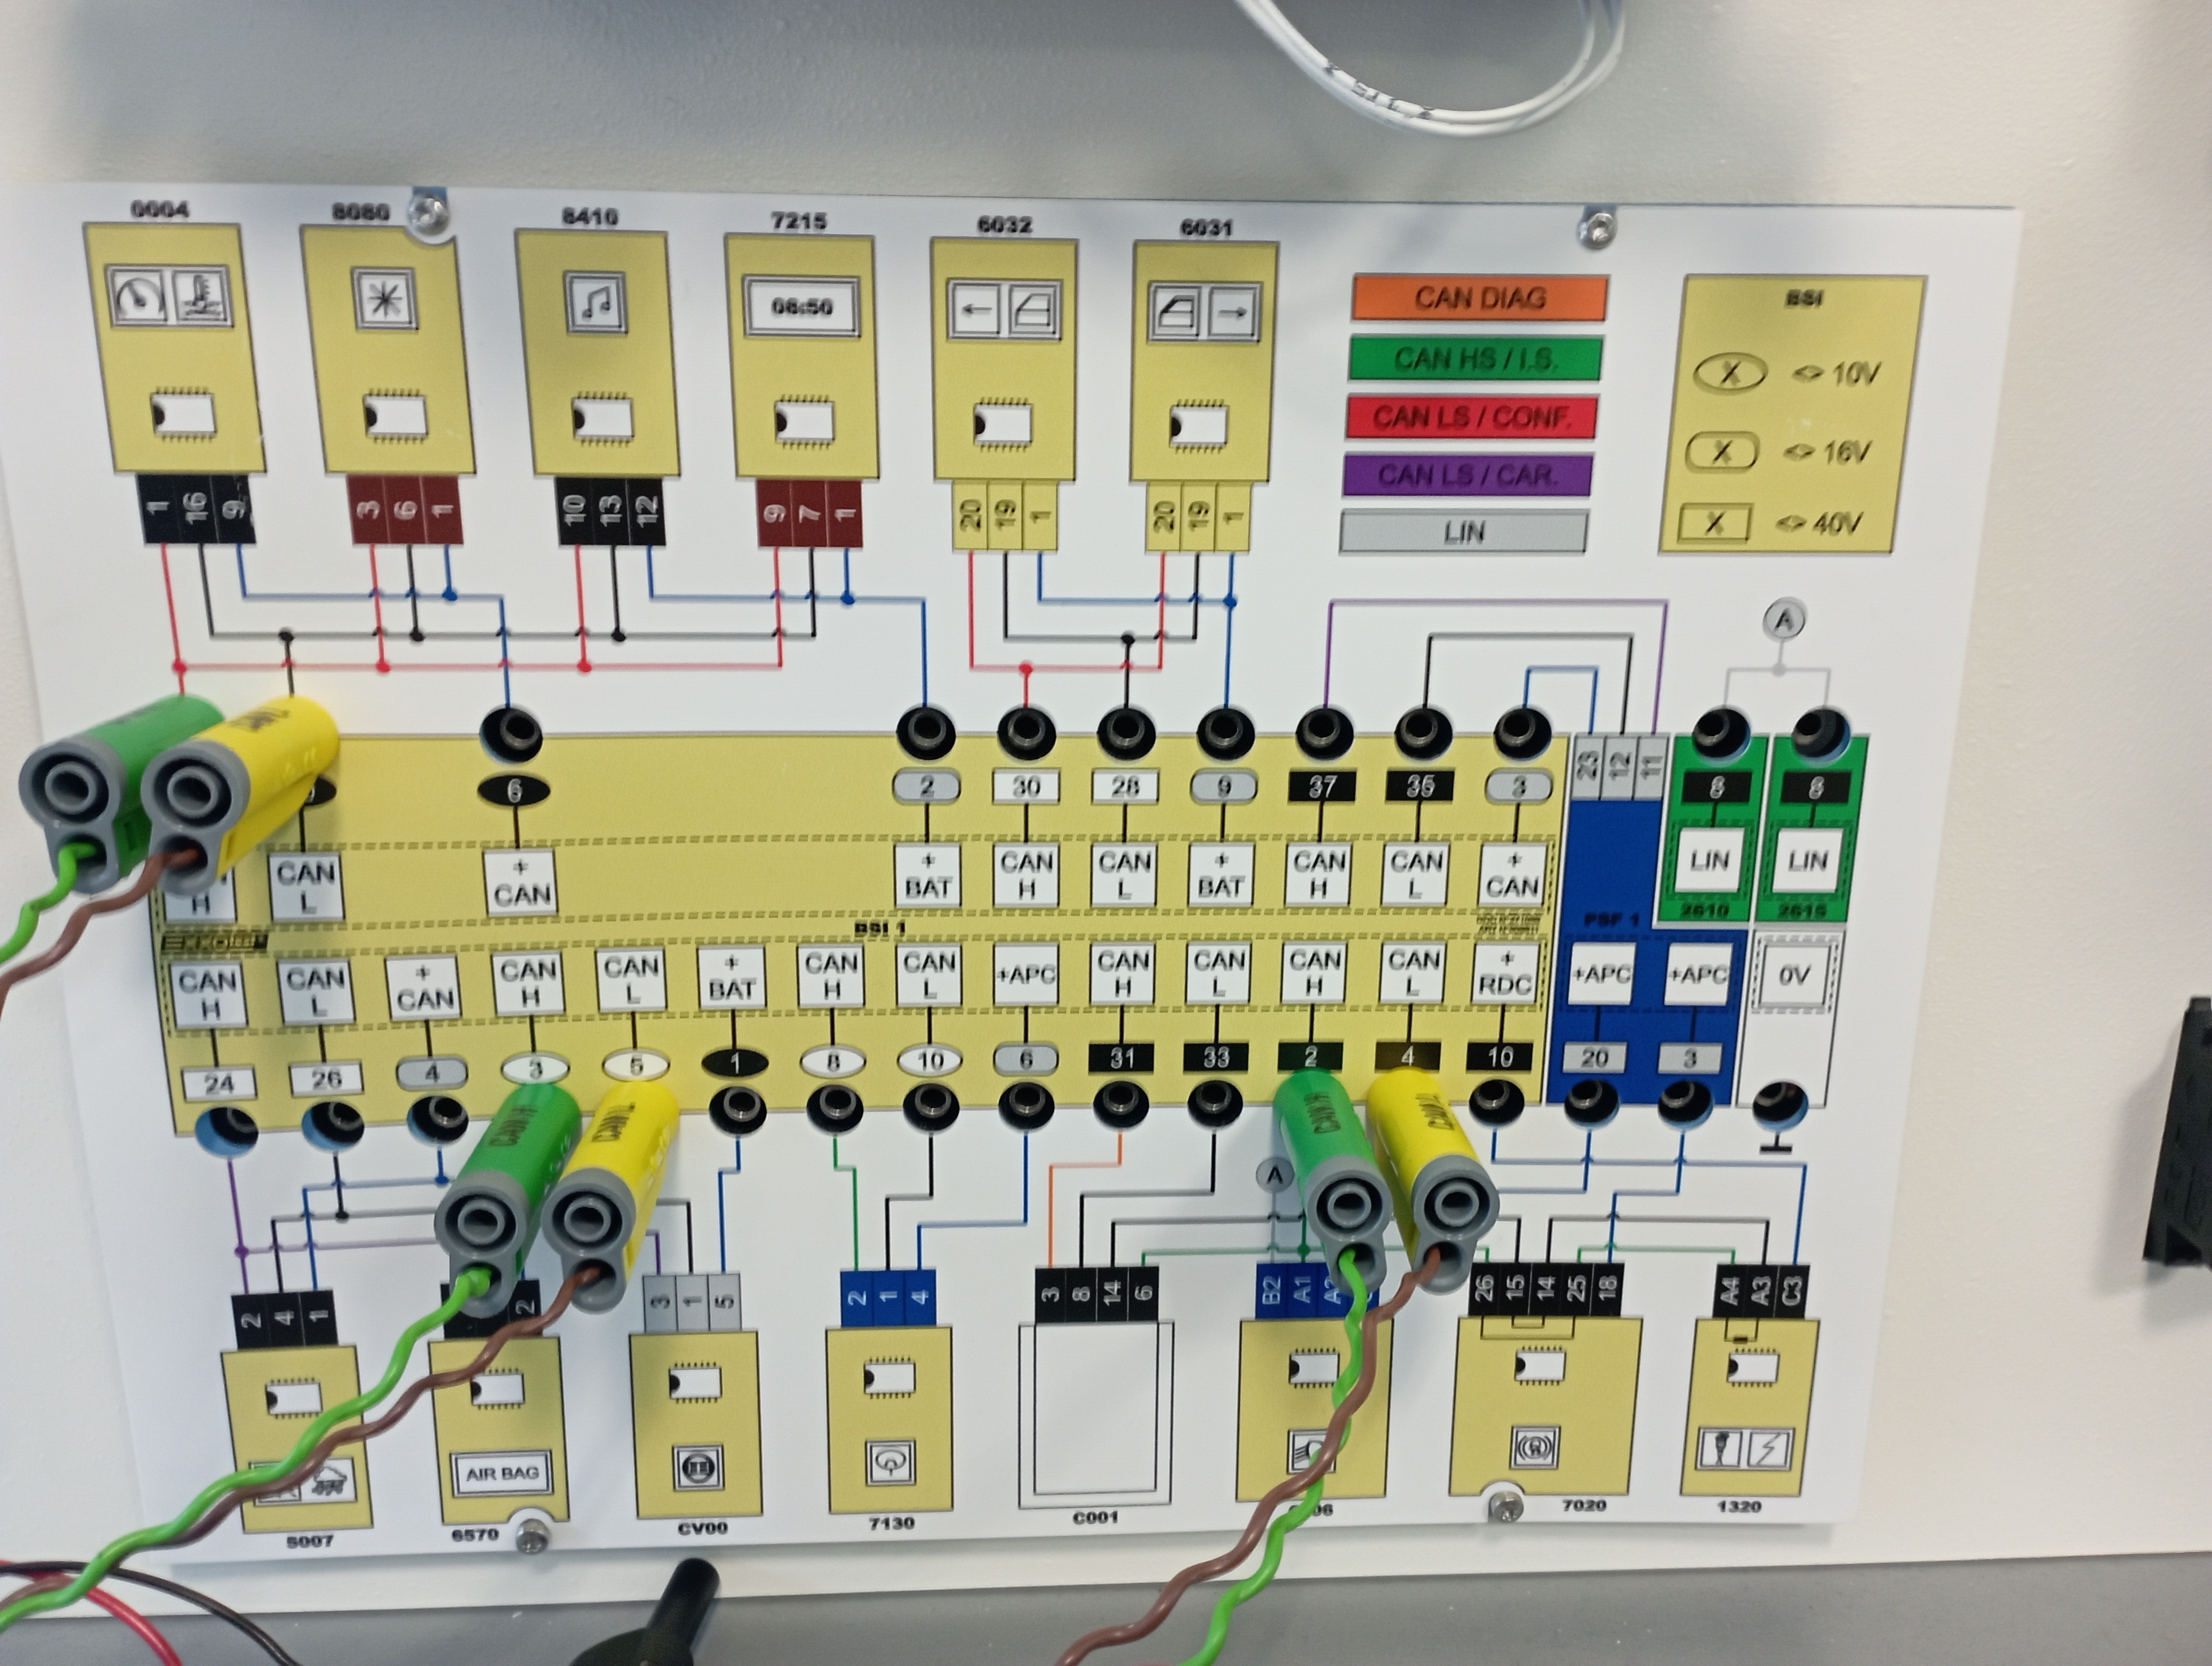
\includegraphics[width=.6\textwidth]{./images/tableau_interface.jpg}
    \caption{Illustration des branchements sur la plaque de la maquette.}
    \label{fig:tableau_interface}
\end{figure}

\begin{figure}[H]
    \centering
    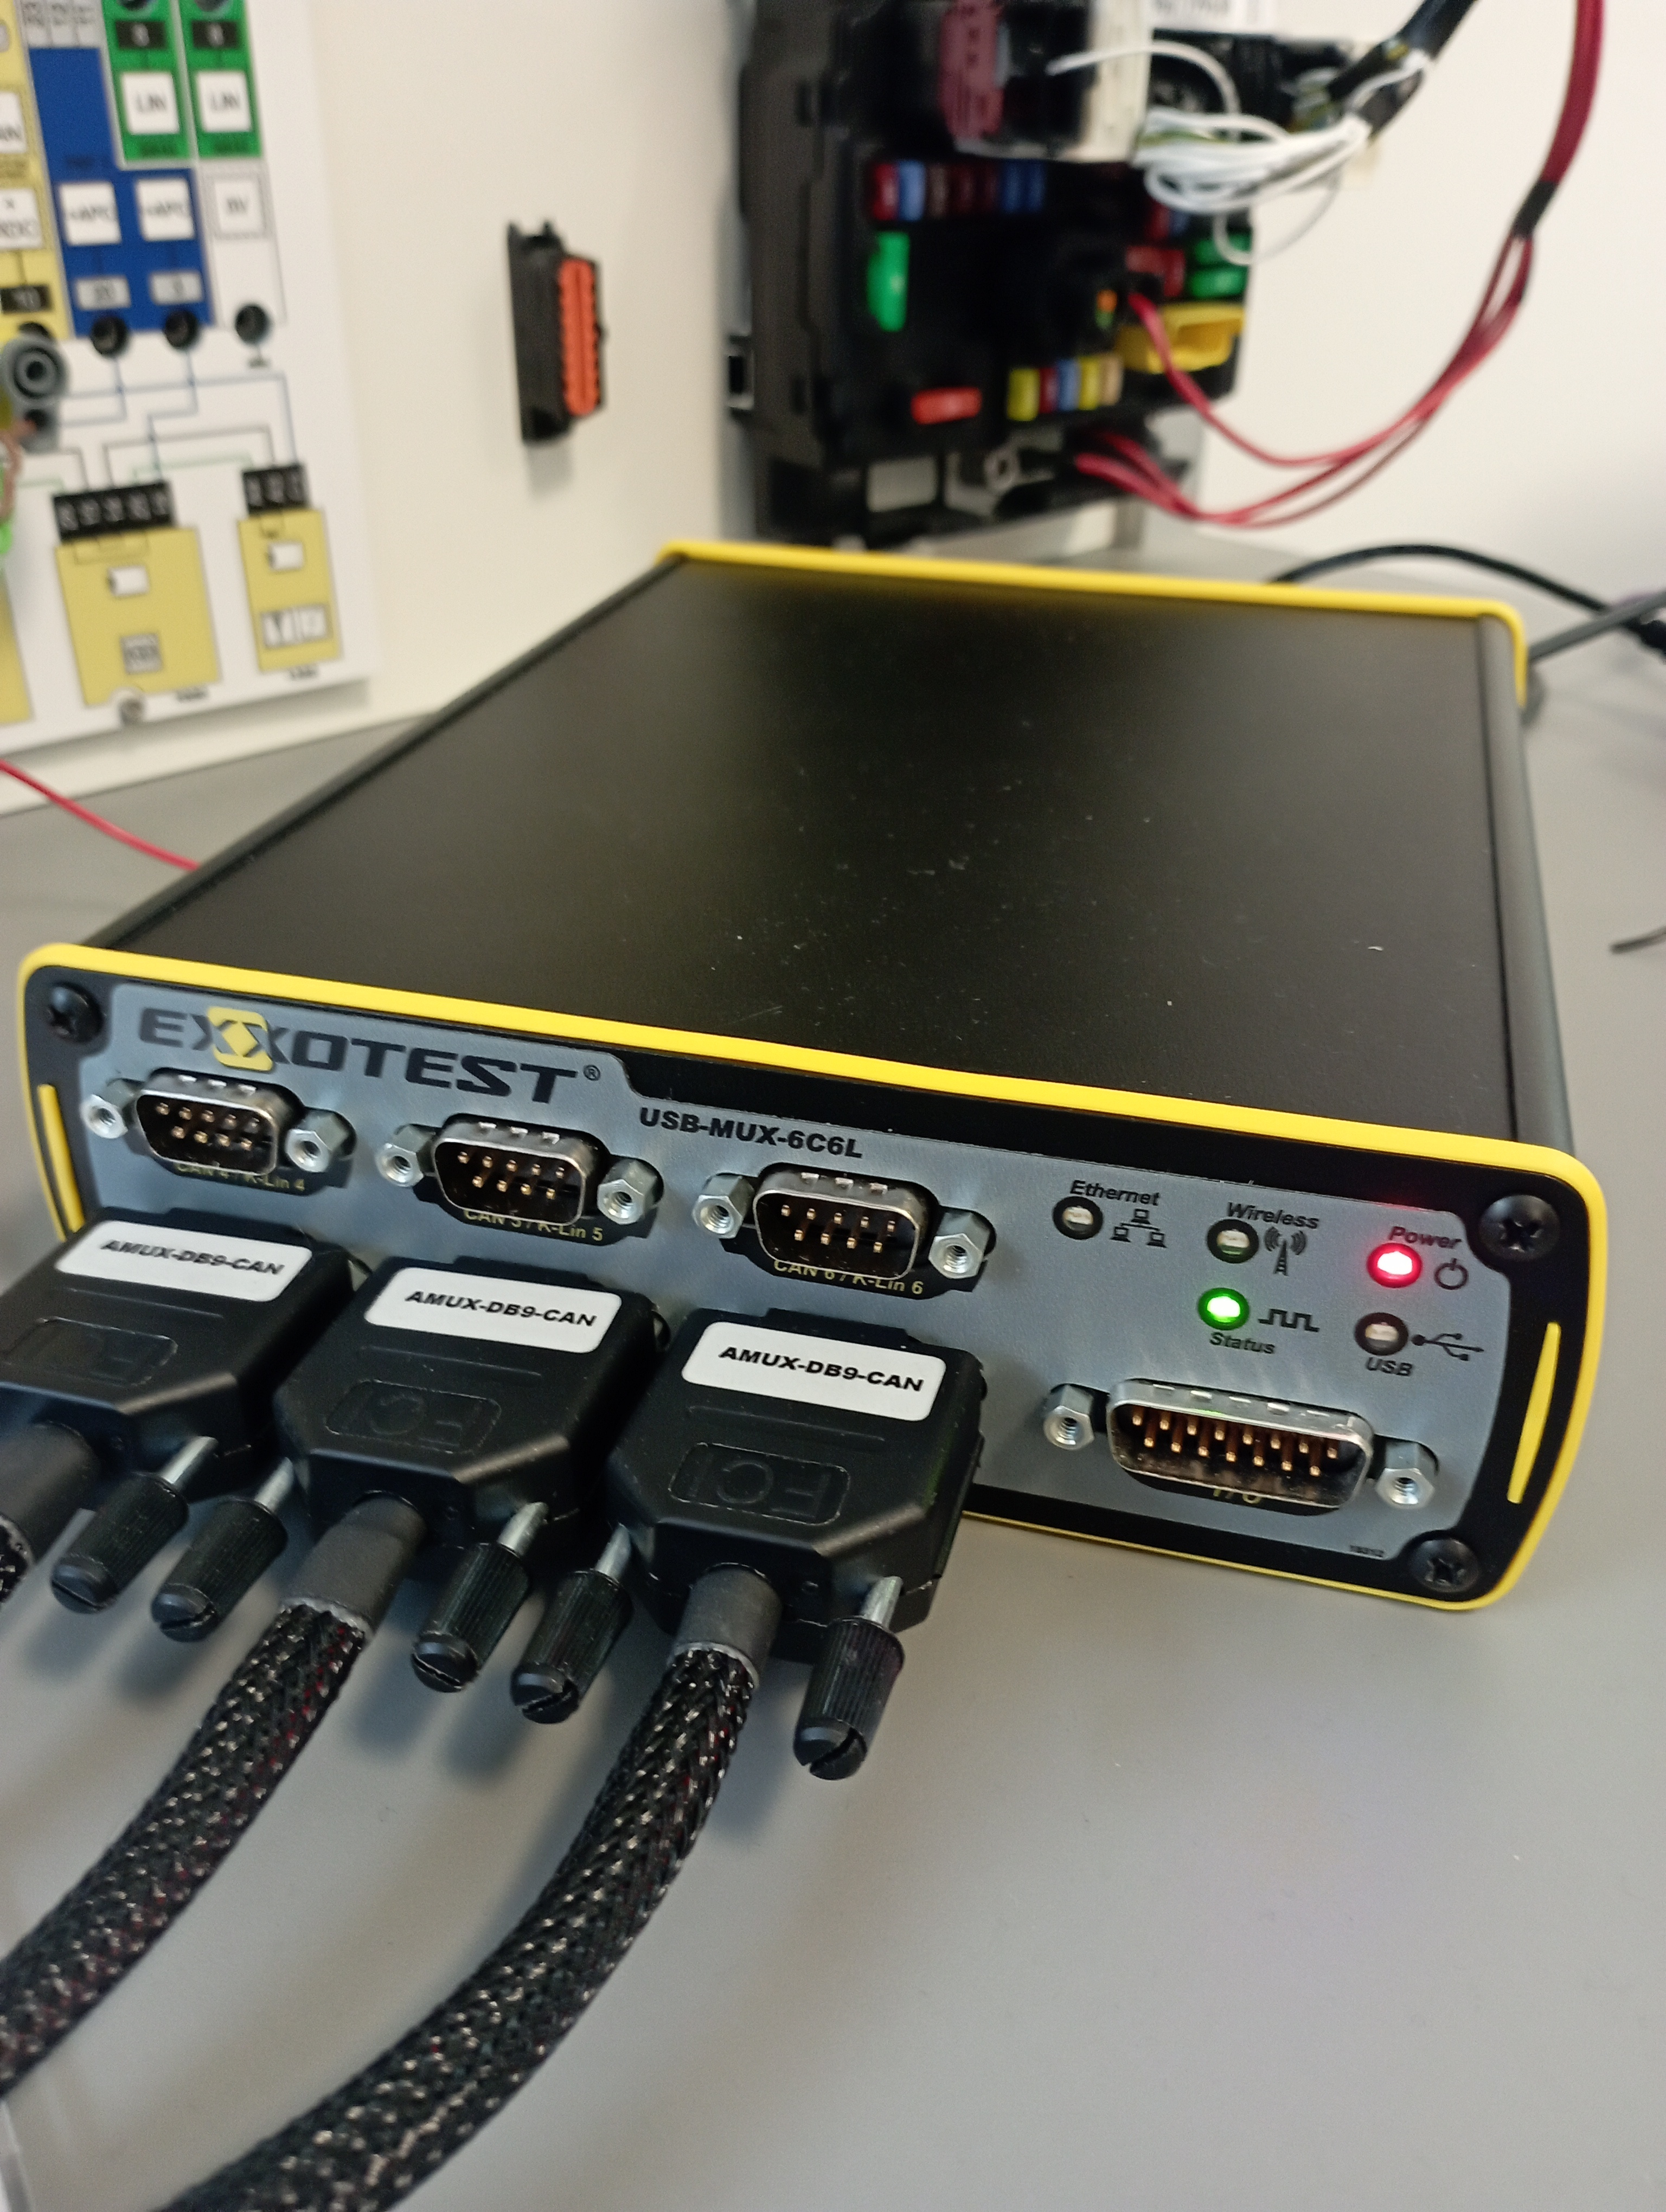
\includegraphics[width=.6\textwidth]{./images/boitier_usb.jpg}
    \caption{Illustration du boitier USB-MUX-6C6L.}
    \label{fig:boitier_usb}
\end{figure}

\subsection{TP3}\label{sec:annexeA:TP3}

\begin{figure}[H]
    \centering
    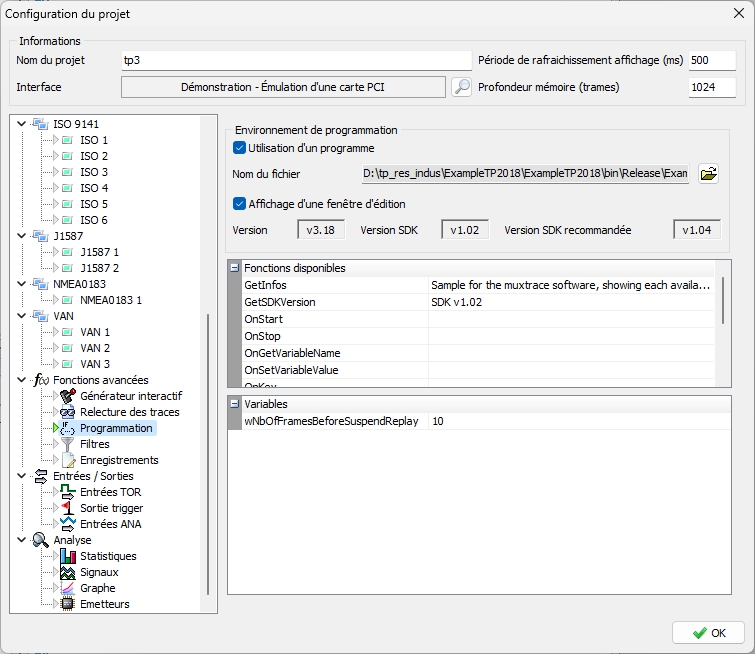
\includegraphics[width=.7\textwidth]{./images/Muxtrace_programmation_configuration_res_indus_31_01_2024_ubs_lorient_M1SESI.png}
    \caption{Configuration supplémentaire du projet pour ajouter l'archive .dll afin de réaliser le test réel vitesse-volume.}
    \label{fig:conf_additional_real_limit_vitesse}
\end{figure}

\begin{figure}[H]
    \centering
    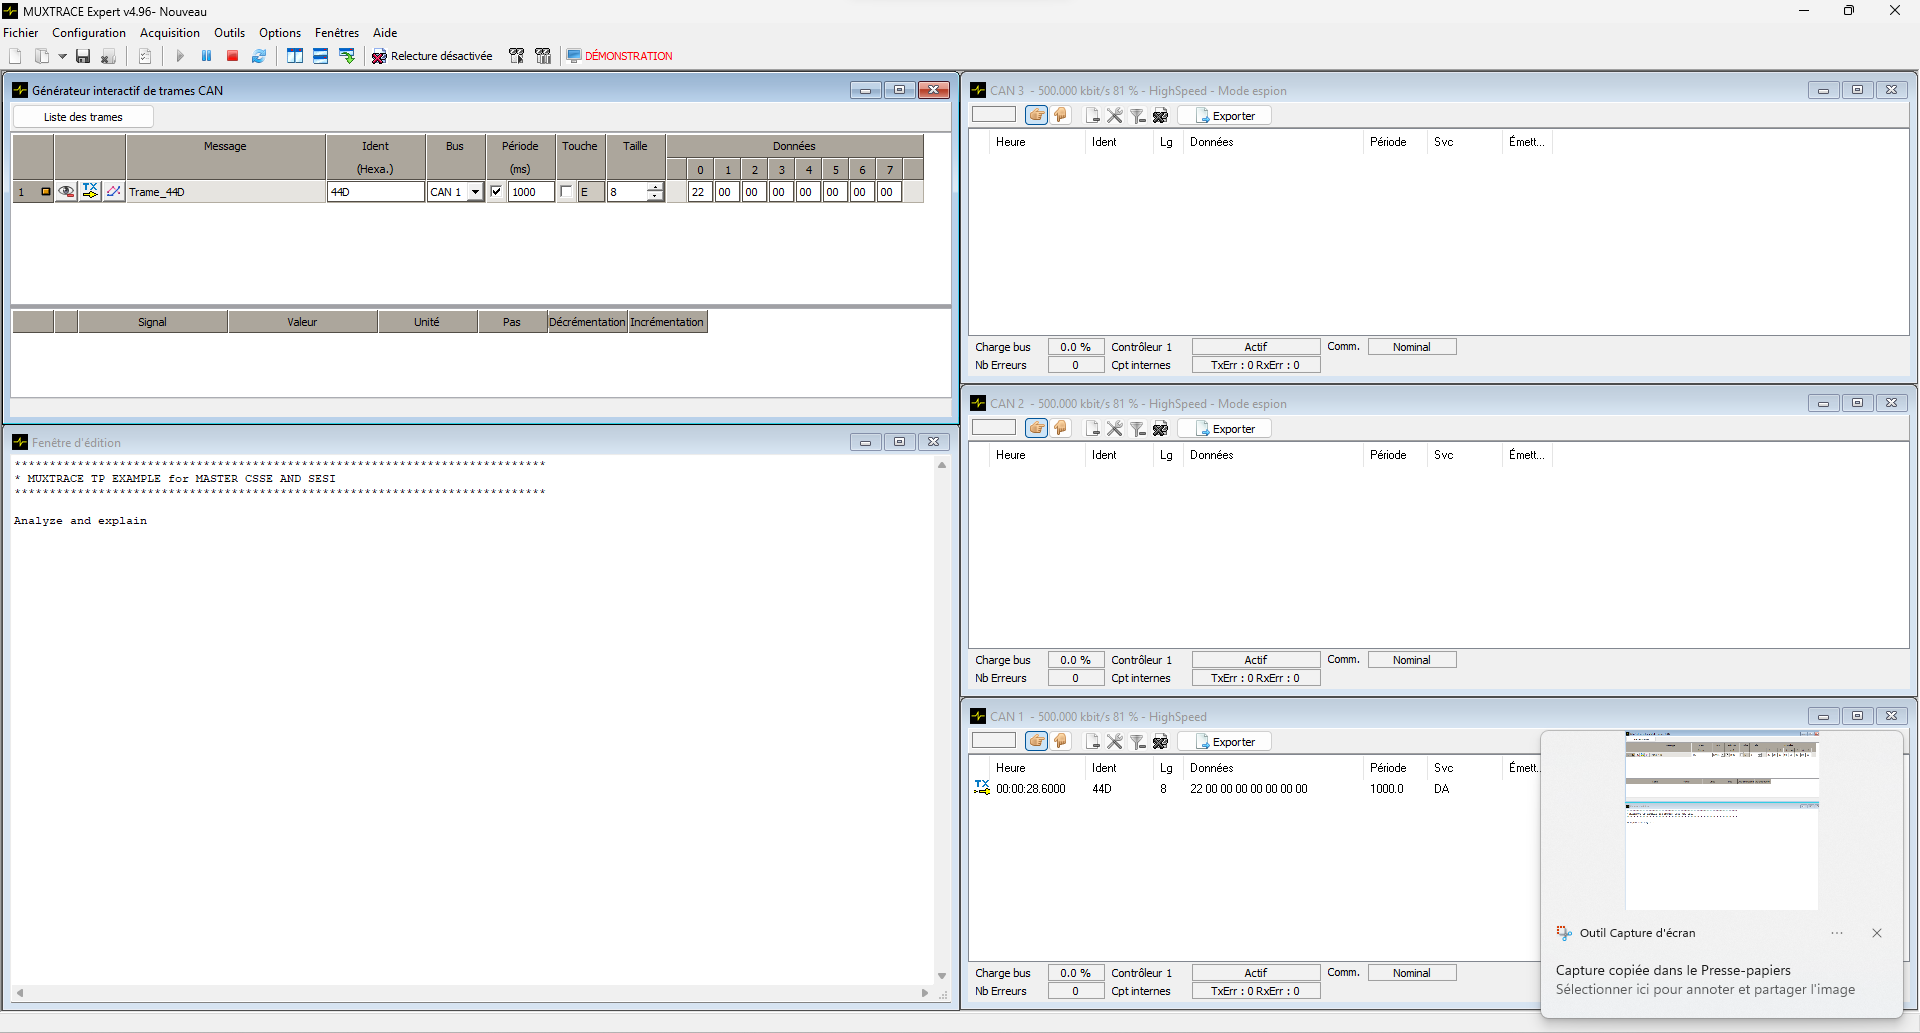
\includegraphics[width=.7\textwidth]{./images/test1.png}
    \caption{Test local avec une vitesse inférieure à 100 km/h. Trame de volume (ID 44D) par défaut 22.}
    \label{fig:test_local_1}
\end{figure}

\begin{figure}[H]
    \centering
    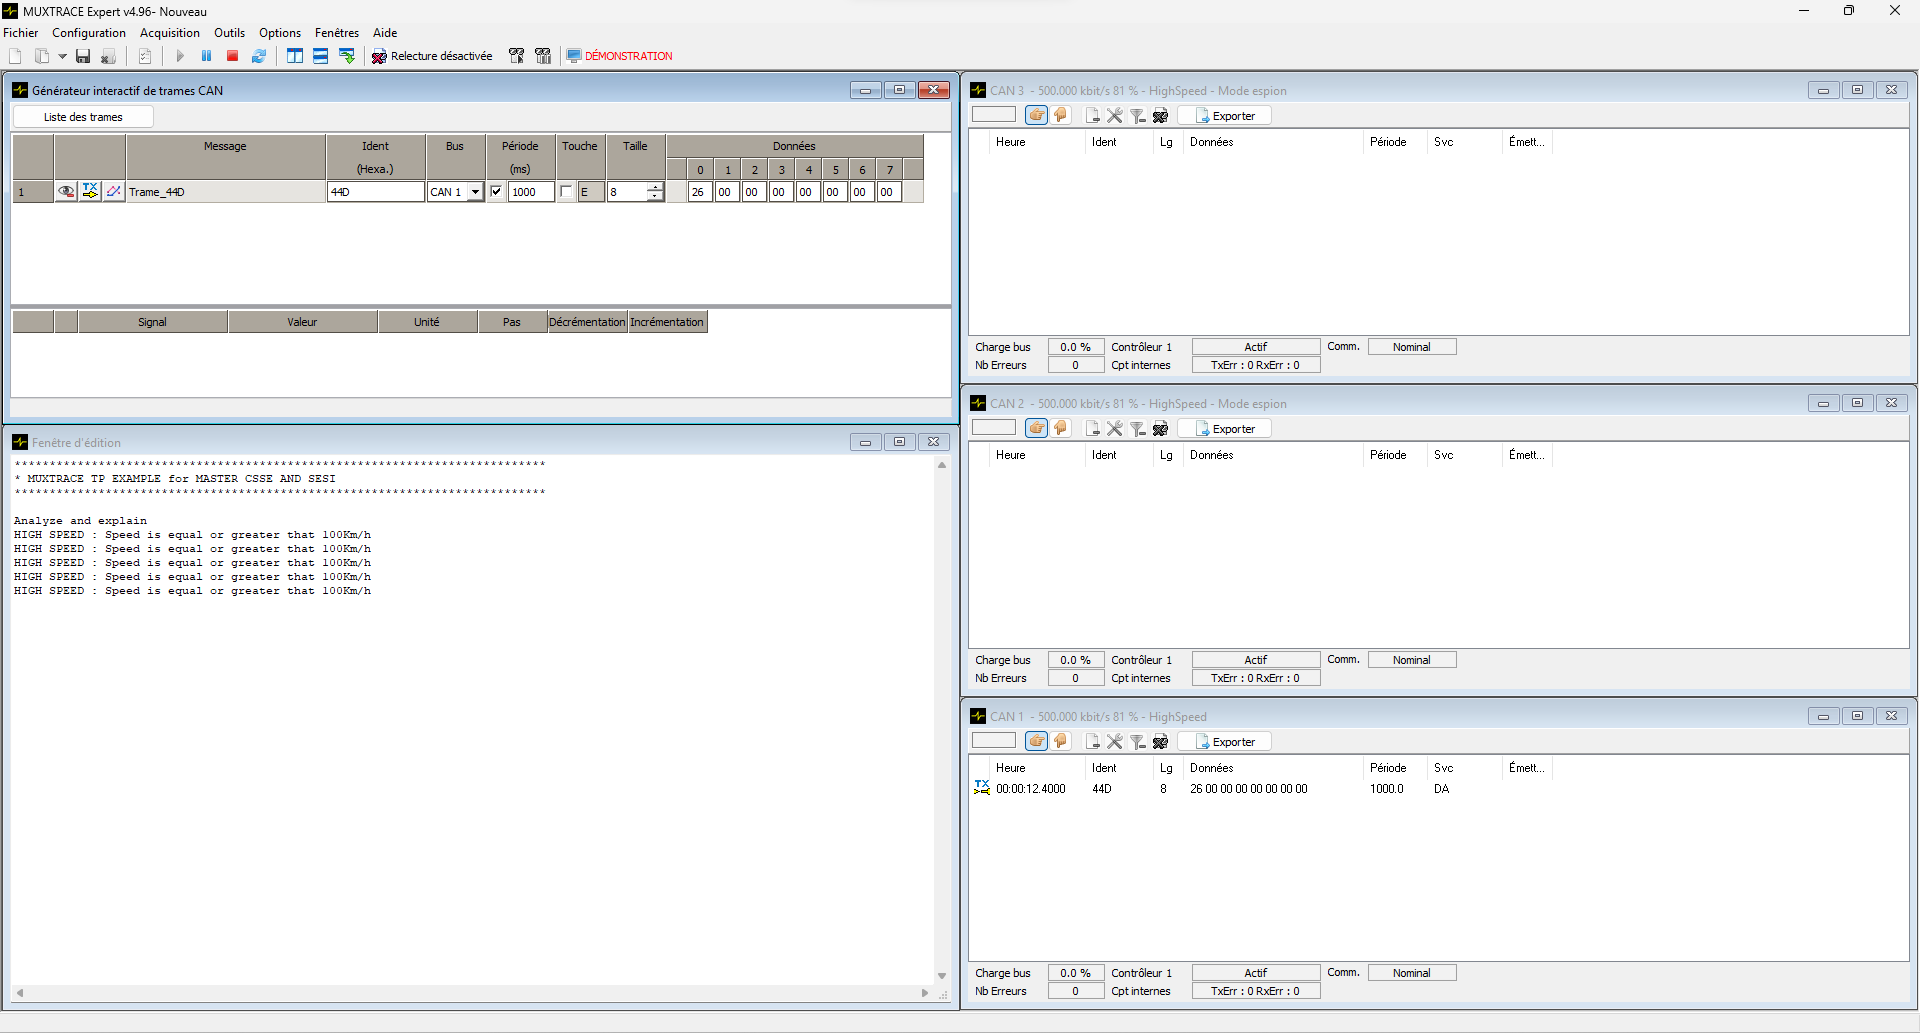
\includegraphics[width=.7\textwidth]{./images/test1_2.png}
    \caption{Essai local avec une vitesse supérieure à 100 km/h, noter le message de débogage et la valeur de la trame 44D (volume) passe de 22 à 26.}
    \label{fig:test_local_2}
\end{figure}

\begin{figure}[H]
    \centering
    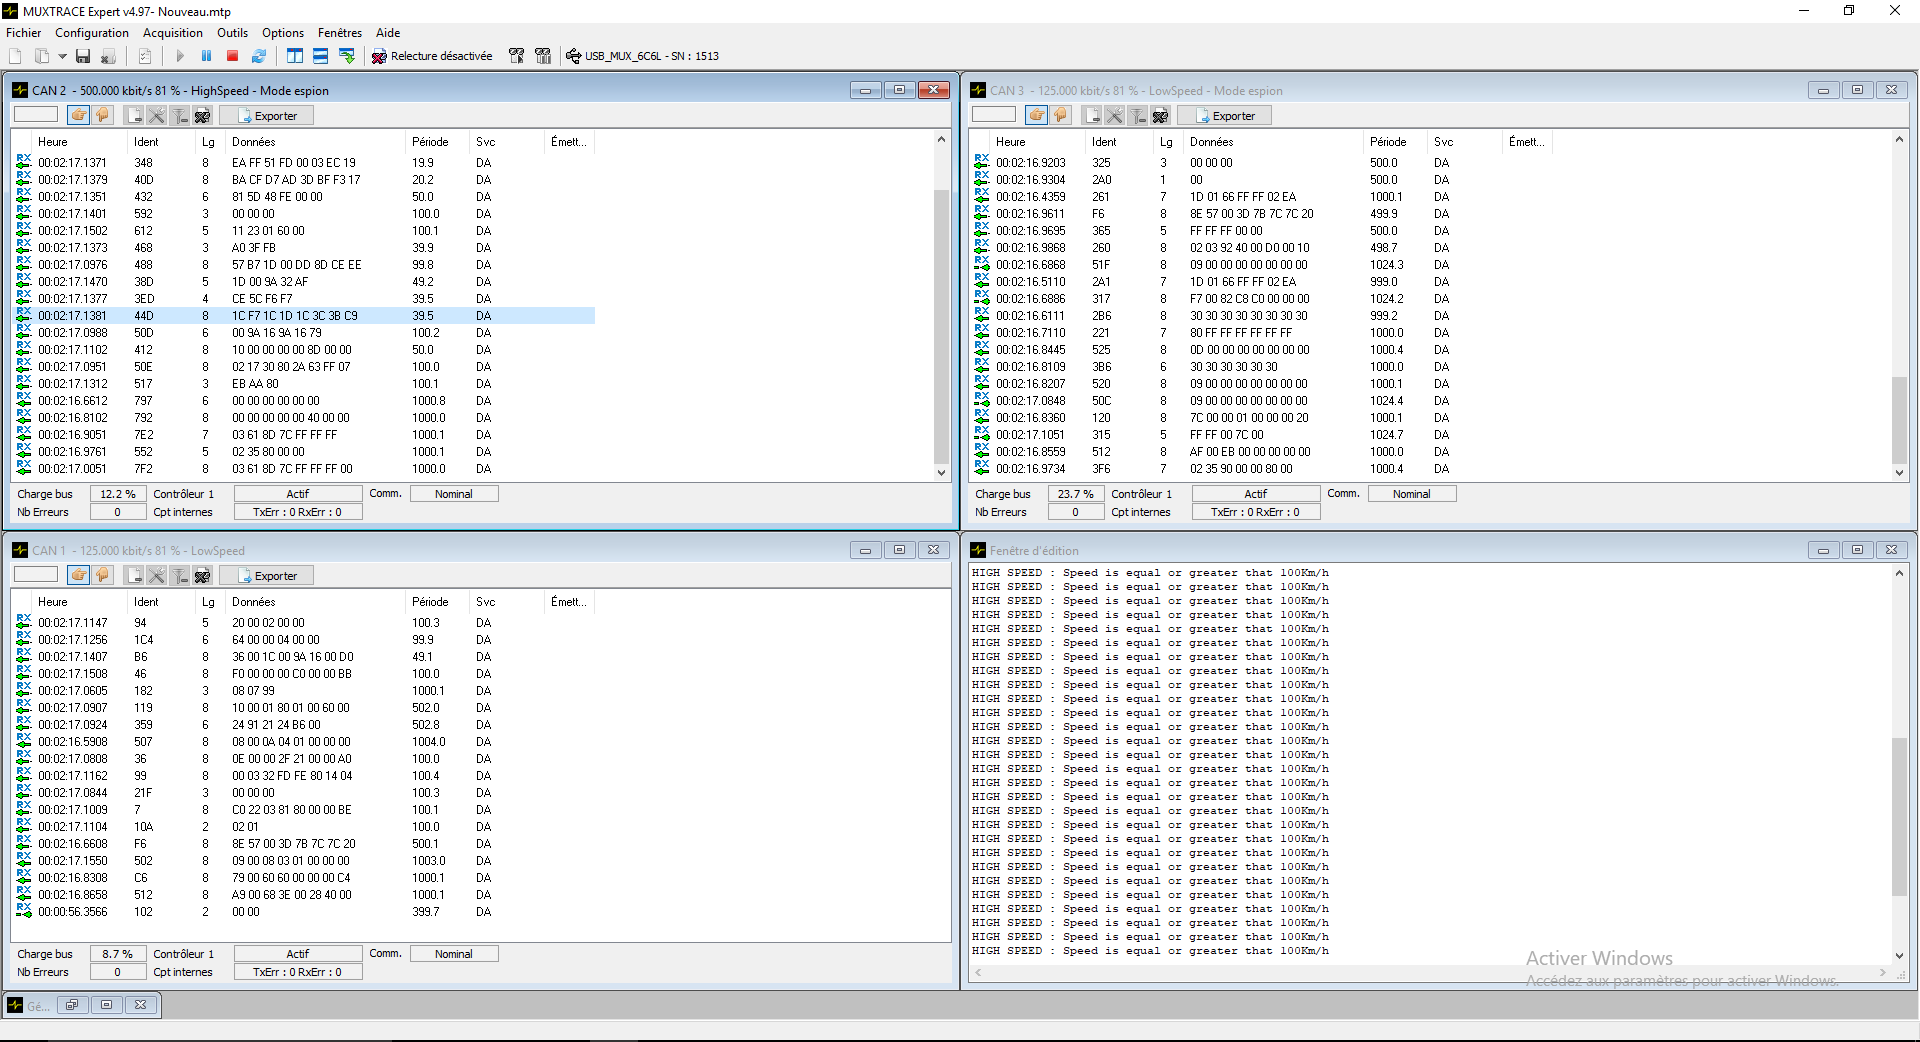
\includegraphics[width=.9\textwidth]{./images/Real_Limit_vitesse.png}
    \caption{Illustration du test vitesse-volume réel}
    \label{fig:real_limit_vitesse}
\end{figure}

\pagebreak

\section{Annexe B : Code Snippets}\label{sec:annexeB}

\lstinputlisting[language=C++, caption={Fonction OnEvent original.}, label={lst:onevent}]{./code_snippets/OnTimer_default.cpp}

\lstinputlisting[language=C++, caption={Fonction OnCanEvent modifie.}, label={lst:oncanevent}]{./code_snippets/OnCanEvent_mod.cpp}

\end{document}